
\chapter{Proof-of-Turn}
\label{chap:PoT}
In most of the mentioned \gls{CM}s extrinsic incentives, like tokens of cryptocurrencies
(\citet[4]{Butijn.2020}; \citet[3]{Khan.2020} \citet[85]{Kraft.2016}; \citet[4]{Nakamoto.2009}), are given.
The \gls{PoT} approach assumes intrinsic motivation instead, in this regard comparable to \gls{CM}s based on voting.
Still, the upper level software is assumed to offer enough incentives.
Nevertheless, mechanisms need to be established, which prevent nodes to behave hostile or malicious. \\
\gls{PoT} is guided by the business case of bringing \textit{turn based games} onto \gls{BC} infrastructure.
On a high level of abstraction, \gls{PoT} reminds of the round robin
nature of 'Token-Ring Local-Area Networks' (\citet{Bux.1989}; \citet{Ergen.2004}).
Although sticking to the phrase '\textit{turn}', this chapter abstracts from the gaming context.
Still, the \textit{turn}, as emphasized in its name, is the key factor of \gls{PoT} and therefore described first (Figure \ref{fig:TheTurn}).
\begin{figure}
	\centering{
		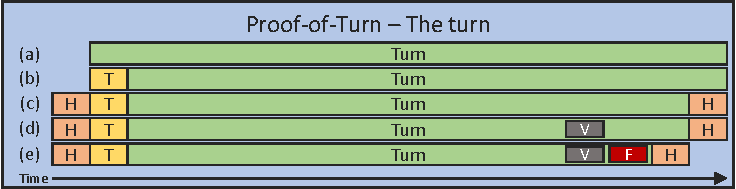
\includegraphics[width=.95\linewidth,keepaspectratio=true]{contents/images/TheTurn}
		\caption{The turn}
		\label{fig:TheTurn}
	}
\end{figure}
In the most basic approach, each node awaits its turn, which is a predefined time slot in the round robin procedure (Figure \ref{fig:TheTurn}, (a): \textbf{Green turn}).
Derived from the gaming context, on the one hand, a turn may last only ten seconds.
On the other hand it is assumed that a turn will commonly last several hours or days.
By the time a node has its turn, it is called the \gls{LN}. \\
Moreover, the turns are assumed to enable \textbf{transition times} between the turns (Figure \ref{fig:TheTurn}, (b): \textbf{Yellow T}).
The transition times are supposed to be set to a constant
value of \textit{five} seconds, no matter how long the turn.
It is essential for transition times to last long enough to prevent network related race conditions \cite[75]{NetzerR.H.B..1992}.
Consequently the last \gls{LN} and its successor do not assume to be the \gls{LN} at the same time, preventing mutually exclusive forks. \\
In a more advanced case, the \gls{LN} and its successor both sign an arranged \textbf{handover-block} to seal the transition (Figure \ref{fig:TheTurn}, (c): \textbf{Orange H}).
This raises the security for the \gls{LN}'s successor to write to the latest branch(/fork) whilst ensuring the \gls{CF} for the \gls{LN}'s written data. \\
Additionally, once finished writing all data, the \gls{LN} may undertake a \textbf{network vote} (Figure \ref{fig:TheTurn}, (d): \textbf{Gray V}).
The vote asks upon the compliance of all in this turn published blocks.
Each node which received the vote call, raises the possibility for \gls{CF} as the possibility for a fork, leaving out the \gls{LN}'s data, is diminished.
Additionally, each positive reply increases the possibility for posted data to reach \textit{effective \gls{CF}}
(Section: \hyperref[sec:CFandBFT]{Consensus finality and Byzantine Fault Tolerance}) even before the \gls{LN}'s writing permission has ended.
If some data does not pass the vote, the \gls{LN} has the opportunity to revise the posted data until the turn's time slot is over.
A revision is supposed to only append blocks, setting things right.
Forks are prevented. \\
Once the \gls{LN} considers its turn to be finished, a \textbf{finalizing block} may be created,
which terminates the turn even before the designated time slot has passed (Figure \ref{fig:TheTurn}, (e): \textbf{Red F}).
Consequently, a \textit{finalizing block} is the 'soft version' of a 'hard and explicit' handover enforced by the end of the turn's time slot. \\
During its turn, the \gls{LN} is free to post all desired data.
In the first place the amount of data is only limited by the turn time and the \gls{LN}'s physical computation capacity.
Therefore, the turn's time slot has to be designed appropriately to ensure that all data can be written.
The latter is dependent on the upper level use case.
The bare minimum for data/blocks to be accepted is complying with \gls{BC}'s base structure
(Figure \ref{fig:BlockchainStructure}) combined with the \gls{LN}'s (valid) signature.
\begin{figure}
	\centering{
		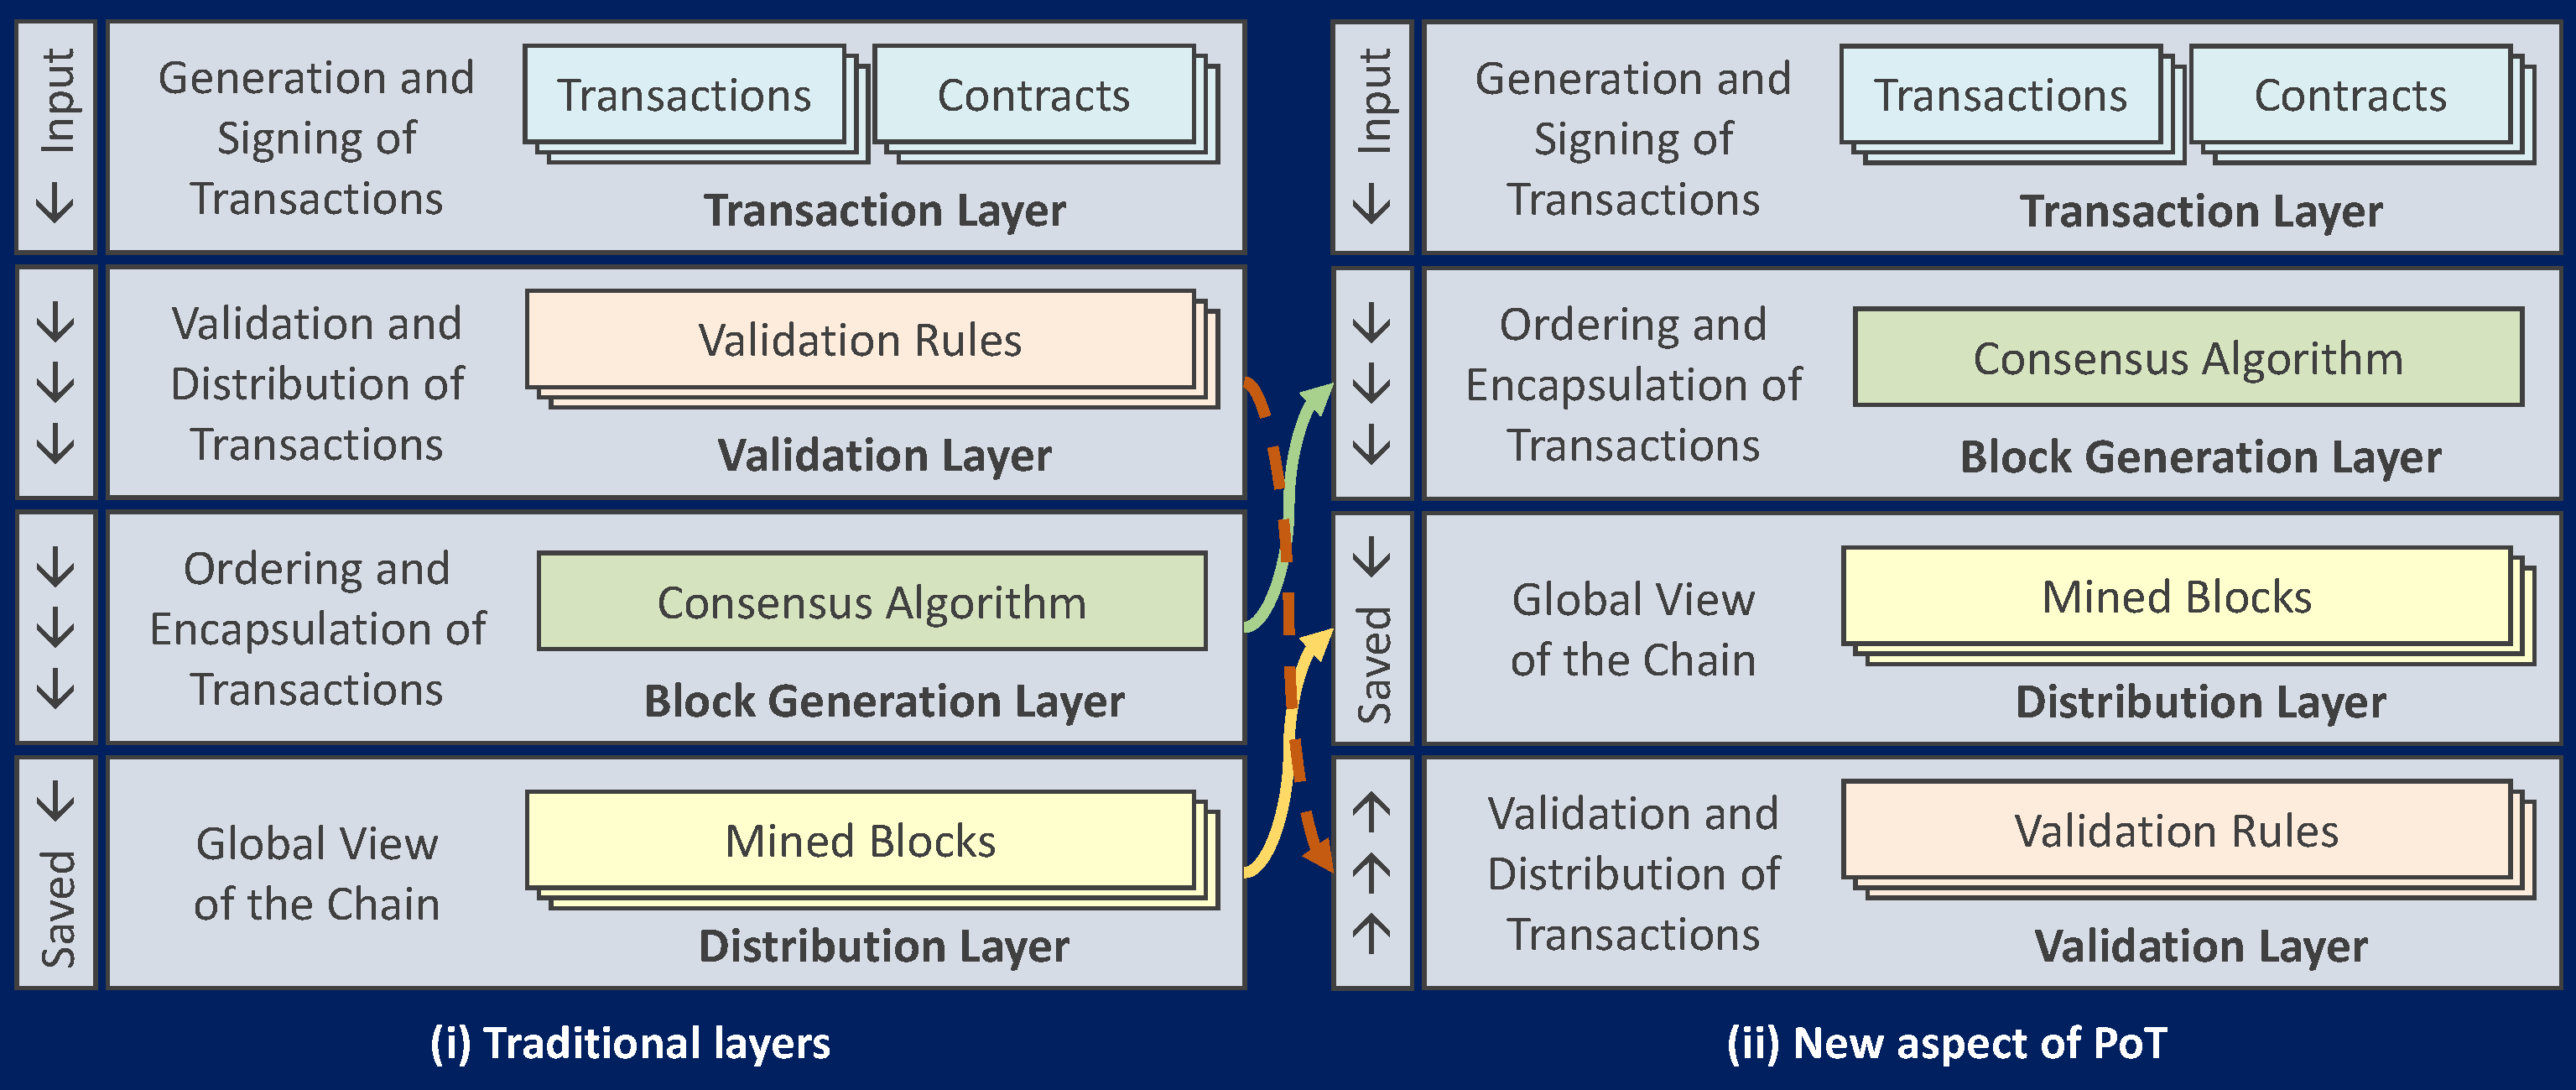
\includegraphics[width=.95\linewidth,keepaspectratio=true]{contents/images/BlockchainLayersPoT}
		\caption{Layers in PoT (Adapted from  \citet{Oliveira.2019})}
		\label{fig:BlockchainLayersPoT}
	}
\end{figure}

\noindent At this point, the four layers of \gls{BCT} (Figure \ref{fig:LayersOfBlockchains}) are used in \gls{PoT} as well.
Depending on the attitude, on the one hand, one can argue that the validation is only conducted by the \gls{LN} and then directly pushed into the distribution layer.
The argument for this theory is the immediate \gls{CF} of each signed block.
The block is then part of the chain and immutable.
Following the definition, the \gls{CM} ends with the distribution (Figure \ref{fig:BlockchainLayersPoT}: (i)).
On the other hand, \gls{PoT} requires the data to be investigated after being distributed.
The data can not be deleted, but may be invalidated thereafter.
Consequently the validation layer is set last (Figure \ref{fig:BlockchainLayersPoT}: (ii)).
It is assumed that given a proper rule set, the invalidation will never occur.
Nevertheless, the nature of \textit{hidden transactions} may offer constraints to any previously published data (e.g. a node is offline during its turn (benign fault) and cannot reveal critical data) and
therefore raise the possibility of invalidation. \\
Regarding performance, nodes in other \gls{CM}s as \gls{PoW} have to try multiple times to mine a new block.
Comparably, proposing a new block in \gls{PoT} is cheap,
as the \gls{LN}'s fingerprint, derived from private-public key encryption,
on a block is sufficient for proposing the next block into the \gls{BC}.
Hence the runtime of each block's creation in \gls{PoT} is assumed to be $O(1)$. \\
As \gls{PoT} does not tie the \gls{LN}s block creation on mining success,
on-chain improvements like \hyperref[sec:PerformanceImprovements]{'Big block'} are obsolete.
In the first place, it is not distinguished between a \textbf{single block} containing
'all in the turn created data' from proposing \textbf{multiple blocks}.
Here, upper level rules may enforce to propose multiple blocks.
The latter, stems from randomization calls, which have to be finalized in the network,
before the \gls{LN} is allowed to continue its turn. \\
\textbf{\gls{PoT} is fully asynchronous.}
Therefore, in the most basic approach, \gls{PoT} does not allow other nodes to interfere a turn anyhow.
There is no repository for other node's transactions which have to be put into a block by the \gls{LN}.
Nevertheless, to enable randomization, disputes and likewise transactions, which demand consultation, either a fast single purpose round
(Section: \hyperref[sec:ClaimsAndTriggers]{Reveal claims \& trigger events}) has to be conducted
or any side-chain solution (Section: \hyperref[sec:Interoperability]{Interoperability}) may be used.\\
Of course, any time each node may send a direct message to the \gls{LN} to raise a dispute.
The \gls{LN} is supposed to follow \textit{legit disputes} to prevent double work,
invalidation, or (worst case) being sentenced with a handicap or any harder punishment by the whole network based on upper level rules.
Still, the \gls{LN} may decide to follow the validated (but not yet voted upon) dispute or ignore it.
The latter may lead to an invalidation of the affected data and a possible reset of multiple turns.
As the \gls{LN} has an intrinsic incentive for progress, it will most likely give in to a dispute call and raise a network vote upon the issue. \\
The \gls{PoT} concept is resembling to multiple, already existing approaches:
\begin{enumerate}
	\item \textbf{\gls{PoA}} assumes only a few nodes of the network to operate as writing/publishing nodes.
	The two clients \textit{Aura} and \textit{Clique} from the general \gls{PoA} are pretty similar to \gls{PoT}
	as they both elect one primary writing node, which is changing after a defined time slot \cite[2]{Angelis.2018}.
	Whilst \textit{Clique} allows multiple nodes to write simultaneously granting priority for the blocks written by the \gls{LN},
	\textit{Aura} and \gls{PoT} assume exactly one node to be allowed to write/publish data.
	But Aura votes for every emitted block directly,
	which leads to instant \gls{CF}, but slows down the system itself.
	Voting upon newly published blocks is optional in \gls{PoT} and generally tied to finalizing a turn.
	Additionally, \gls{PoT}'s \gls{LN} is generally not assumed to write data originating from other nodes.
	
	\item \textbf{\gls{PoP}} and \gls{PoT} are both primarily located in the gaming context.
	
	\item \textbf{\textit{Multichain}} uses a loose round-robin procedure, whilst \gls{PoT} enforces a strict round-robin sequence.
	\textit{Multichain} prevents nodes to write until a defined percentage of other nodes has written any block \cite[7-8]{Greenspan.2015}.
	If all the nodes allowed to propose a block remain silent, \textit{Multichain} freezes.
	The possibility freeze is not applicable in \gls{PoT} due to strict (maximum) time slots for each node's turn.
	Hence, the network has to wait until the next \gls{LN}'s successor becomes the \gls{LN}, but the network does not stall completely.
	
	\item \textbf{\gls{PoET}} uses exact timing to determine the next writing/publishing node.
	Although \gls{PoT} uses transition times to prevent the need for exact timing hardware,
	timing plays an important role passing the right for writing/publishing data to the \gls{BC}.

	\item \textbf{Vote based consensus} decides on each block or writing node separately.
	The common ground with \gls{PoT} arises in special occasions e.g. disputes
	which leaves all nodes to vote to either accept or invalidate a previous block or transaction.
\end{enumerate}
\noindent Due to its stiff progression of \gls{LN}s, \gls{PoT} is considered
to be used in \textit{private} or \textit{public} environments,
operated in permissioned or hybrid manner (Table: \ref{tbl:BlockchainNetworkTypes}).
If nodes joined and left the network in high fluctuation (e.g. in a permissionless environment),
\gls{PoT} would stall from absent nodes and may break its intended performance characteristics. \\
In the following, mechanisms and characteristics of \gls{PoT} are described:
\begin{enumerate}
	\item \gls{CF} and \gls{BFT} are discussed.
	\item General \hyperref[sec:Peering]{peering} of nodes is addressed.
	\item The classification into the \hyperref[sec:CAPtheorem]{CAP Theorem} is given.
	\item Passing turns and handling of possible forks are covered using \hyperref[sec:TransitionBlocks]{transition blocks}.
	\item \hyperref[sec:Interoperability]{Interoperability} with other \gls{BC} \gls{CM}s is described.
	\item Measures regarding \hyperref[sec:PeerFluctuation]{peer-fluctuation} are presented.
	\item Implications of \hyperref[sec:ClaimsAndTriggers]{trigger events} are shown.
	\item \hyperref[sec:FurtherCharacteristics]{Further characteristics} are given.
	\item Possible \hyperref[sec:AttackVectors]{attack vectors} are described.
	\item \hyperref[sec:Limitations]{Limitations} of \gls{PoT} are addressed.
\end{enumerate}



\FloatBarrier

\section{Consensus finality \& Byzantine Fault Tolerance}
\label{sec:CFandBFT}

Each \gls{LN} is supposed to validate its blocks following the given \gls{SC}s.
As stated before the blocks, written to the \gls{BC} by the \gls{LN}, meet \gls{CF} instantly - no consultation is needed.
The price to be paid for this fast-forward solution, is the possibility of a block to be invalidated thereafter.
Here it has to be differentiated between \textit{legal enhancements} (legally \textbf{added} to the \gls {BC})
and \textit{legal transactions} (legal \textbf{content} of the transactions).
In \gls{PoT} \textit{legal enhancements} of the blockchain structure (appending any block) meet \gls{CF} instantly.
The capsuled \textit{transactions}, may be invalidated sometime later.
The latter does not happen in the most \gls{BCT} algorithms like \gls{PoW}, as each transaction has to be open to everyone in the network to  pass the validation.
Unfortunately, the nature of game play sometimes prevents the direct detection of fraudulent (hidden) transactions.
In a worst case scenario the node itself - due to other hidden transactions - does not even know that its own transaction is invalid.
The latter has to be prevented by upper level rules.
Once a fraud \textbf{can be detected} by another node, a 'non action' being the \gls{LN}, equals a consent.
Hence, after data has passed $\geq 50\%$ of the nodes without intervention - no matter obviously fraudulent or not - the data can be seen as \textit{effectively consensus final}.
The $\geq 50\%$ refer to active nodes.
After all, this drawback - \gls{CF} vs. effective \gls{CF} - has to be accepted.
At the latest, when the writing node becomes the \gls{LN} again, it can be sure the published and revealed data is accepted without dispute.
Consequently, the scenario of a \textit{computational super power} recalculating the
chain - as possible in \gls{PoW} \cite[8]{Nakamoto.2009} - is not applicable in \gls{PoT}.
\gls{PoT} does not follow the \hyperref[LongestChainRule]{Longest Chain Rule}.\\
Additionally, voting to kick nodes out of the network which behave \textit{obviously hostile} is possible.
For both, voting for 'invalidation of any block' and 'kicking due to hostile behavior', a vote process has to be conducted.
The threshold, used in such a vote, is supposed to be set to $\geq 50\%$, but can be shifted as needed.
It is important that the following is known: \textbf{this threshold marks the \gls{BFT} for the whole algorithm}.
Consequently, the \gls{BFT} of \gls{PoT} remains implementation dependent as stated in table \ref{tbl:SumConsensusMechanisms_3}. \\
Game play related \gls{BFT}, as dependent on card draw mechanics, are explicitly not part of the \gls{PoT}-specific \gls{BFT} performance.
Last, to prevent any node flooding the \gls{BC}, it has to be considered whether a limit of written blocks/data is set for each turn.
Generally a limit is not recommended, as first bloat blocks may exceed the limits and
second disputes votes and following inflicted handicap upon hostile nodes can easily be conducted in a retrospection.



\FloatBarrier

\section{Peering}
\label{sec:Peering}
Data needs to be distributed through procedures and processes in the network.
Although the following section is about networks and peering, specific details of the TCP/IP- as well as the
OSI-model (\citet{Forouzan.2003}) are not discussed. \\
As the \gls{CM} manages new transactions decentralized, passing them trough the layers (Figure \ref{fig:BlockchainLayersPoT}), the whole network and its state is not (always) updated on every attached node until a block can be considered \gls{CF}.
Those transactions are previously, encapsulated in mined blocks (\citet{Butijn.2020}; \citet{Khan.2020}; \citet{Nakamoto.2009}), pushed towards the ledger from each node within the network.
In the most \gls{CM}s each node can always push a block into the network legally (\citet{Khan.2020}).
Hence, the (active) ledger is represented by many nodes simultaneously.
On the contrary, a pull(only)-mechanism to fetch updates would generate an enormous amount of network traffic as every node has to pull from every other node constantly.
Given the number of nodes, $n$, the number of pull requests for updates would scale by '$f(n) = n^2$'.
In a binary world, using a push-mechanism for new data is evidently the right choice
as the next block's origin node can be any network node.
Nevertheless, popular clients as Ethereum, Hyperledger Fabric and Corda mix both mechanisms \cite[6]{Daniel.2019}.
Still, literally, a node has to push hard to fight its data into the ledger. \\
In contrast, in \gls{PoT}, the (active) ledger is only represented by one node.
Only the \gls{LN} is allowed to push new transactions.
Thus, push- and pull-mechanisms are generally possible (as well) and described in detail.
Nevertheless, before digging deeper, it has to be distinguished between two scenarios, \textbf{consultationless} and \textbf{consultationfull}.
On the one hand, a \textbf{consultationless} network would be a shared storage wherein data is pushed only for others to be seen.
No node has a desire to change other node's data.
There is no reason for disputes or spontaneous interactions - such as triggers or throw in transactions.
On the other hand, a \textbf{consultationfull} network is assumed to utilize randomization calls, votes,
disputes as well as spontaneous interactions multiple times during a full (round robin) network round. \\
Moreover, the nodes are supposed to be loosely coupled, as players of games may quit (the game) or shut down their client.
Additionally, high mobility of nodes may hinder static network addresses and connectivity.
Hence, a broadcast in dedicated (static) sub networks is not applicable. \\
Last, permanent direct, linked connections are subsequently excluded due to possibly high numbers of nodes.
Therefore, more than five nodes are expected. \\
The literature describes peering mechanisms of \gls{BCT} only on seldom occasion referring to single transactions \cite[4]{Daniel.2019}.
Consequently push-mechanisms from an emitting node into the (whole) network are supposed to be common,
whilst pull-mechanisms exceeding \gls{SC}s could not be found in the literature.
Consequently the literature lacks an overall picture using 'only a pull-Mechanism' or 'only a push-mechanism'. \\
Given these assumptions, a sample pull-mechanism and a sample push-mechanism are described:



\subsection{Pull-Mechanism} \label{def:PullMechanism}
As stated, the decentralized nature of \gls{BCT} prevents frequently 'full-network' pull-mechanisms generally.
Nevertheless, in the special case of \gls{PoT}, the \gls{LN} circles,
alternating from node to node, due to the round robin procedure.
Hence, the source for the latest update is defined by time.
Consequently, nodes may pull from the latest \gls{LN} directly or from its predecessor to prevent interventions of the \gls{LN}'s turn.
\begin{figure}[!b]
	\centering{
		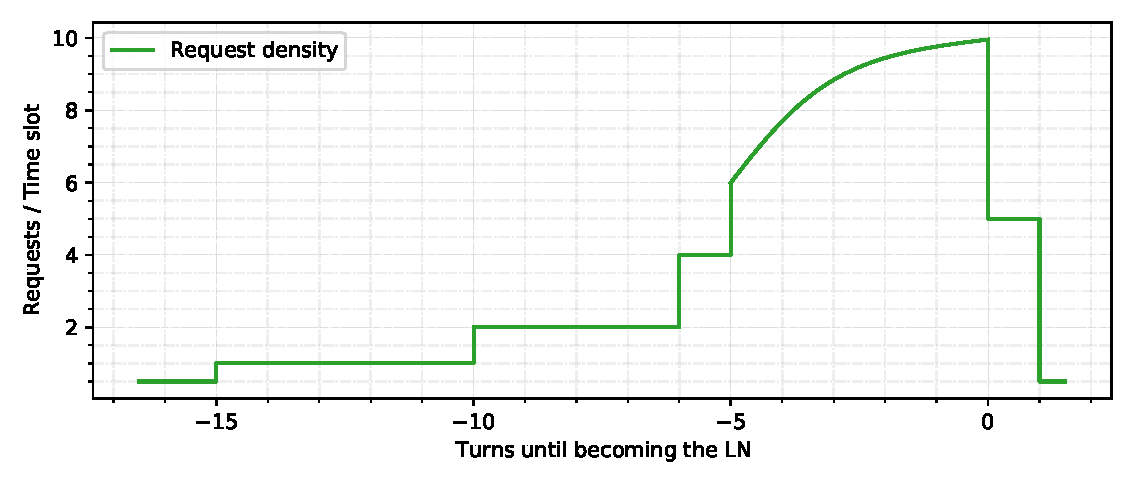
\includegraphics[width=.95\linewidth,keepaspectratio=true]{contents/images/PeeringByPulling}
		\caption{Sample 'peering by pulling'-strategy}
		\label{fig:PeeringByPulling}
	}
\end{figure}
Hence, the number of requests is tremendously reduced. \\
The following description is therefore set in a \textbf{consultationless} use case.
The nodes are lazy and try to pull seldom to \textit{reduce network traffic}.
Hence, each node is just waiting for its own turn.
A node missing its own turn is considered a worst case scenario.
Therefore, if a node expects to have its turn soon, it becomes more active.
A sample pull strategy is given in figure \ref{fig:PeeringByPulling} and different node's behaviors are described in the following. \\
On the y axis, the pull strategy in 'requests per time slot' is given.
For the sake of tangibility, first, 60 minutes is set as a turn's time slot ($t = 60 min$).
Second, the network consist of '$n=50$' nodes.
Third, the network is not stiff, as 'ending a turn prior to its maturity' is possible. \\	
This pull strategy is designed to be constraint to the node's distance to its next turn.
Along the round robin alternation, the node will have its turn again and again in the multiple of $n$.
But the number of turns until the next slot of being the \gls{LN} has to be within
'$x < n$'\footnote{\hspace{0.1cm}Depending on the base index, '$x \leq n$' is applicable as well}.
Predecessors of the \gls{LN} are not directly reset - hence '$x > 0$' is possible - and consequently a \textit{sample overflow} is set to ten ($n*1/5 = 10$).
Hence, most network nodes ($n*4/5 = 40$) assume to have a negative index.
The range of x can be described as:

\begin{center}
	$-n*(4/5) \leq x \leq n*1/5 = -40 \leq x \leq 10$.
\end{center}

\noindent The used index overflow is implementation dependent. \\
Effectively, assuming from a time measurement, that nine turns need to be conducted until becoming the \gls{LN}, offers the input '$x = -9$' on the x axis.
Following figure \ref{fig:PeeringByPulling}'s graph, '$x=-9$' leads to \textit{two} pull requests per turn (time slot) or likewise \textit{one} pull request ($p$) each 30 minutes.

\begin{center}
	$p = t/f(x) = 60min/f(-9) = 60min/2 = 30min$
\end{center}

\noindent Given these assumptions, the following cases (\textbf{A} to \textbf{E}) are distinguished:
\begin{enumerate}
	\item \textbf{Node A} is half way through the round robin
	
	\begin{center}
		$x = -(n/2) = -(50/2) = -25$
	\end{center}
	
	and looking forward to its next turn, which is more than 15 turns away (Figure \ref{fig:PeeringByPulling}: '$x < -15$').
	The sample pull strategy function returns '$y = 0.5$' for values below '$x = -15$'.
	One could say that node \textbf{A} is conducting in a 'network deep sleep', as it pulls only every second turn:
	
	\begin{center}
		$p = t/f(x) = 60min/f(-25) = 60min/0.5 = 120min$
	\end{center}

	Nodes do not ask node \textbf{A} for updates, as they prefer to pull from nodes, which are assumed to just have finished their turn (e.g.: $ 1 \leq x \leq 10$), likewise node \textbf{E}.
	Obviously, node \textbf{A} does not assume to have its next turn soon.
	Even if some peers finished their turns early, a seldom pull request is sufficient to not miss the time slot for becoming the \gls{LN}.
	Hence, an update is requested after \textit{two time slots have passed} (Figure \ref{fig:PeeringByPulling}: '$x < -15$').
	The request follows the logic of the \gls{BPMN} diagram (Figure \ref{fig:PeeringPullProcedure}).
	As turns can be ended prior to its maturity, node \textbf{A} only has a scale guess on the recent \gls{LN}.
	Consequently, node \textbf{A} tries to calculate the \gls{LN} heuristically, assuming no prior prematurely turnover.
	Hence node \textbf{A} requests its updates from the node, which is assumed to have its turn right now (here: node \textbf{D}).
	If node \textbf{D} is the \gls{LN}, it is free to either directly provide the update or refer to an already updated node (e.g. node \textbf{C} or node \textbf{E}).
	The latter shall prevent node \textbf{D} from being bothered during its turn. \\
	In the \textbf{best case}, although targeting the \gls{LN}, node \textbf{A} does not consult node \textbf{D}, but node \textbf{E} instead.
	Although node \textbf{E} is not the \gls{LN} anymore, it has just finished its turn and replies the request offering the latest version of the \gls{BC}.
	In the \textbf{worst case}, no answer is given at all, as node \textbf{D} is offline.
	Node \textbf{A} therefore asks node \textbf{D}'s predecessor (node \textbf{D+1}) and node \textbf{D}'s successor (node \textbf{D-1}), one after another.
	Except the \gls{LN} all nodes are assumed to be willing to provide updates immediately as
	shared data is predisposed to reveal flaws and advances progress.
	Node \textbf{A}'s requests are conducted in both directions until an appropriate answer is received.
	A pull request from itself is obviously skipped.
	In the \textbf{cases in between}, neither node \textbf{D} nor node \textbf{D-1} are targeted by the pull.
	Although data is received, the new information implies that the round robin procedure was (way) faster than expected.
	From the received update, node \textbf{A} can extract the timestamp from the last legal transition block.
	With this information it can recalculate the heuristic.
	Using this knowledge, node \textbf{A} may restart the process directly or wait until its next request trigger.
	
	\item \textbf{Node B} is approaching its turn and assumes to be eighth in line ($x = -8$).
	Consequently, the sample pull strategy function (Figure \ref{fig:PeeringByPulling}) causes node \textbf{B} to perform requests each 30 minutes:
	
	\begin{center}
		$p = t/f(x) = 60min/f(-8) = 60min/2 = 30min$
	\end{center}
	
	In regards of a full round, node \textbf{B} assumes to have its next turn somehow soon.
	Additionally, node \textbf{B} is not consulted by other nodes and utilizes the same procedure as node \textbf{A} (Figure \ref{fig:PeeringPullProcedure}).
	
	\item \textbf{Node C} is almost at its turn and knows to be first in line ($x = -1$).
	Whilst the pull requests increased during the last time slots continuously (Figure \ref{fig:PeeringByPulling}: See '$-5 \leq x < 0$'), node \textbf{C} tries to establish a stable, linked connection to the \gls{LN}.
	Once successful, node \textbf{C} does not need to repeatedly request for updates.
	Node \textbf{C} is only consulted by other nodes in exceptional cases - e.g. other nodes do not reach the \gls{LN} (node \textbf{D}) or its predecessor (node \textbf{E}).
	Node \textbf{C} awaits to become the the \gls{LN}.
	
	\begin{figure}
		\centering{
			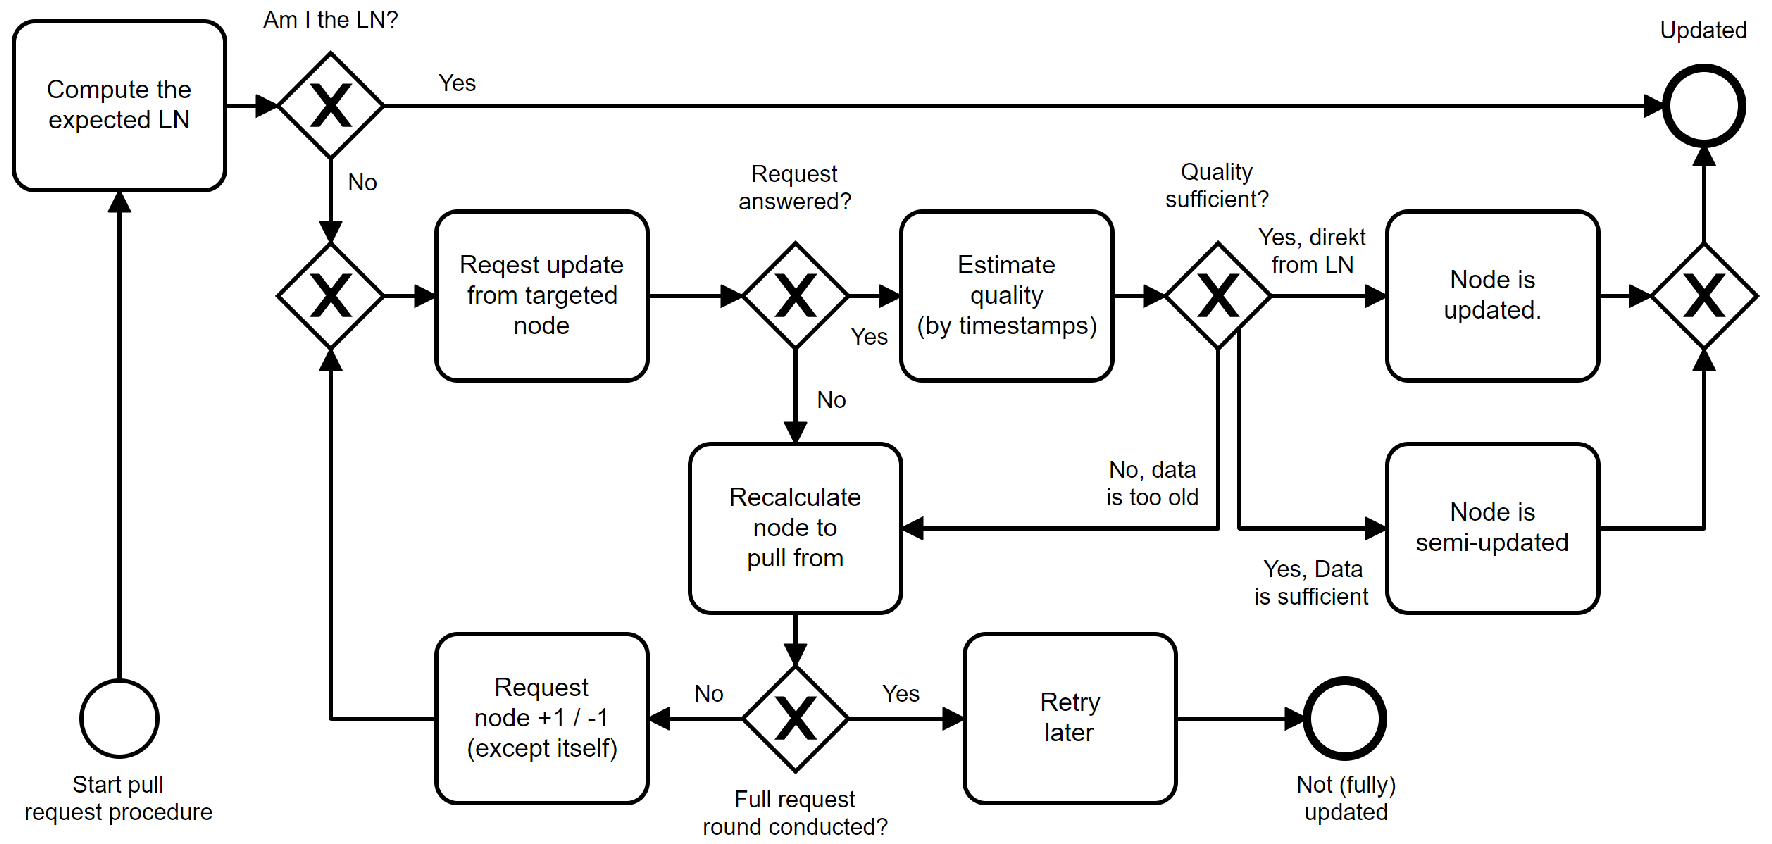
\includegraphics[width=.95\linewidth,keepaspectratio=true]{contents/images/PeeringPullProcedure}
			\caption{Pull request procedure}
			\label{fig:PeeringPullProcedure}
		}
	\end{figure}
	
	\item \textbf{Node D} is the \gls{LN} and in the middle of its turn's time slot ($x = 0$).
	During the transition, node \textbf{D} received the latest version of the \gls{BC} from its predecessor, node \textbf{E}.
	Consequently node \textbf{D} represents the latest version of the ledger and
	has no need to pull from any other node.
	Therefore the pull procedure is skipped by the first junction of the pull process (Figure \ref{fig:PeeringPullProcedure}).
	Still, a suitable value has to be found which balances between triggering
	the pull procedure too often and loosing connection to the network after the turn.
	All \textbf{four equations} (\textbf{I} to \textbf{IV}) represent the same intention: The \gls{LN} starts pulling from other nodes after its own turn. \\
	Whilst formula (\textbf{I}) does not allow to be calculated (Condition: '$f(0) = 0$'), resulting not triggering the pull process anymore,
	formula (\textbf{II.a}), using a value nearby zero ('$f(x) = 0.\overline{0}1$') increases the pull timer
	tremendously as shown formula (\textbf{II.b}).
	Until the next pull procedure is triggered after one year, many turns will have been missed already.
	Both, (\textbf{I}) and (\textbf{IIa} \& \textbf{II.b}) disconnect node \textbf{D} from the network permanently and are therefore dismissed.
	\begin{center}
		Not applicable: \\
		(\textbf{I}): $p = t/f(x) = 60min/f(0) = 60min/0 = NaN =>$ \textit{no pull} \\
		and \\
		(\textbf{II.a}): $p = t/f(x) = 60min/f(0) = 60min/0.\overline{0}1 = p \to +\infty =>$ \textit{no pull} \\
		- likewise - \\
		(\textbf{II.b}): $p = t/f(x) = 60min/f(0) = 60min/0.0001 = 60,000min >$ \textit{1 year} \\
	\end{center}
	Therefore '$f(0) = 5$' was used in figure \ref{fig:PeeringByPulling}, which can be seen in formula (\textbf{III}).
	Here, node \textbf{D} triggers the pull procedure each 12 minutes until the first junction
	of the \gls{BPMN} diagram (Figure \ref{fig:PeeringPullProcedure}) is answered 'No'.
	\begin{center}
		Applied: \\
		(\textbf{III}): $p = t/f(x) = 60min/f(5) = 60min/5 = 12min$ \\
	\end{center}
	\textbf{Instead}, a ratio could be used to send node \textbf{D} into a 'network deep sleep' as shown in formula (\textbf{IV}).
	The equation changes and uses a quarter round ($n*(1/4)$), constraint to the number of nodes.
	This leads node \textbf{D} to pull after $12.5h$:
	\begin{center}
		(\textbf{IV}): $p = t*(n*1/4) = 60min*(50*0.25) = 60min*12.5 = 12.5h$ \\
	\end{center}
	While node \textbf{D} is not pulling from other nodes, a stable, linked connection with the successor node \textbf{C} is established.
	Frequently node \textbf{D} is asked whether it is the recent \gls{LN}.
	If node \textbf{D} had ended its turn already, it would provide the update.
	The other way around, node \textbf{D} may reference to a likewise updated node, such as node \textbf{E} or node \textbf{C}.
	Once all data is pushed, node \textbf{D} may end its turn early.
	Of course node \textbf{D} is allowed to decide whether it wants to remain the \gls{LN} until the end of its turn's time slot or pass the turn to its successor before.
	An upper level application may incentive node \textbf{D} to pass the turn as fast as possible or prevent prior finalization of its turn.
	A reason against passing the turn ahead of schedule is that the \gls{LN}'s successor is not linked, yet.
	A variable turn time may allow the \gls{LN} to even prolongate its turn's time slot given certain conditions.
	The changing starting times with every prior-finished turn may allow to last a \gls{LN}'s turn until the stiff's end (Figure \ref{fig:TurnEndBeforeMaturity}).
	As the node might assumed to have the start of its turn later on.
	Either first, the node can not be blamed, second the rules stipulate a strict variable plan or third rules enforce online activity and aligned turn times.
	
	\item \textbf{Node E} has just ended its turn.
	The node \textbf{D} has taken the lead and node \textbf{E} will pull again when the trigger (formula \textbf{III} or \textbf{IV}) is activated.
	Node \textbf{E} will reset its index, once it reaches the \textit{sample overflow} ($x=10$).
	Consequently, for it's own updates, node \textbf{E} raises pull to the bare minimum and falls into a 'deep sleep', alike node \textbf{A}.
	Still, the next time slots will consist of many pull requests, which have to provide the latest data.
\end{enumerate}

\noindent Concluding, aiming to optimize network traffic, a pull strategy is supposed to be the most lightweight scenario as nodes are allowed to fall into a 'deep sleep'.
Still the pull strategy function has to be adjusted to the networks needs.
Here both, step function elements (Figure \ref{fig:PeeringByPulling}: '$-5 > x$' and '$x \geq 0$') and continuous function elements (Figure \ref{fig:PeeringByPulling}: '$-5 \geq x < 0$') may be used. \\
Obviously, the drawback of consultationless peering is the loss of short termed answers on behalves of the whole network.
Here, to fix the latter issue, a full network round until a decision is made, would be needed.
A special round for consultation, alike in the subsequent section \hyperref[sec:ClaimsAndTriggers]{Reveal claims \& trigger events}
would breaking the stiff time slots and is therefore not suitable in consultationless environments.
Implications of turns 'ending a turn prior to maturity' will be discussed shortly.
Anyhow, stability can be risen using more linked connections or with a higher density of pull requests. \\
Still, regarding the pull request density on the \gls{LN}, in larger networks this might lead unintentionally,
to several internal, flawed by design, \textit{network/transport-level flooding attacks} \cite[2046]{Zargar.2013}, also known as \gls{DDoS}.
Of course there might be possibilities to reduce the network load on the current \gls{LN},
but updates would still trickle slower throughout the network than push based mechanisms, due to the asynchronous nature of pull timings.	
An issue which has to be covered generally using 'ending a turn prior to maturity', is the handling of nodes which take their turn 'too late, but in time'.
Assuming nodes to stay in a permanent deep sleep until their next turn, only pulling once per round, may be sufficient in stiff environments (Figure \ref{fig:TurnEndBeforeMaturity}: A, Eight stiff turns, green).
But using early turnover (Figure \ref{fig:TurnEndBeforeMaturity}: B), the turns one to six might have been ended that fast, that turn seven did not receive the update in time.
Node six has to wait until node seven believes to have its turn again.
Here, the waiting time (Figure \ref{fig:TurnEndBeforeMaturity}: B, Red) would be long enough to conduct two full turns.
A upper level implementation would need to decide either to skip turn seven or to wait until the regular turn slot has passed.
The latter prevents the round robin to proceed faster.
Nevertheless, a fluid turn time demands a higher density of pull requests.
\begin{figure}
	\centering{
		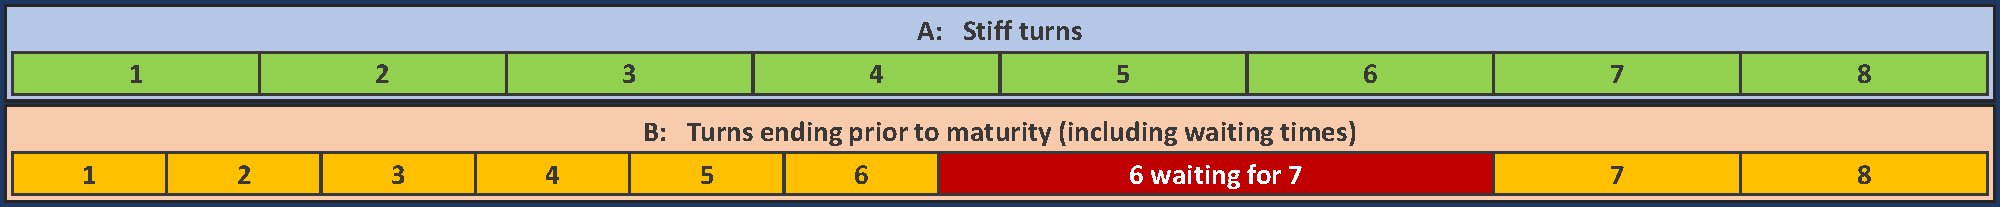
\includegraphics[width=.95\linewidth,keepaspectratio=true]{contents/images/TurnEndBeforeMaturity}
		\caption{Ending turn before maturity}
		\label{fig:TurnEndBeforeMaturity}
	}
\end{figure}


\subsection{Push-Mechanism} \label{def:PushMechanism}
Still in a binary world, in contrast to pull-mechanisms, a push based procedure offers several benefits.
Again no literature regarding (full network) push-mechanism could be found.
Nevertheless, the loose nature of \textit{public permissionless} networks (see table \ref{tbl:BlockchainNetworkTypes})
, e.g. Bitcoin, does not fit the subsequently described, custom tailored push-mechanism for \gls{PoT}. \\
In \gls{PoT}, the \gls{LN} only needs to communicate whenever it is willing to do so.
Consequently, the \gls{LN} is not flooded with several update requests as seen the described pull-mechanism.
Depending on the network size ($n$), in small networks the \gls{LN} may send its data to all peers itself (Figure \ref{fig:PeeringPushMechanism}: A) , using a direct push.
In large networks (e.g.: $n>50$), a mechanism may be established to pipe the updates through \gls{DNs} to reduce the workload for the \gls{LN} (Figure \ref{fig:PeeringPushMechanism}: B).
In this regards, this example uses a '$10x$' scale.
Proceeding, instead of sending an update packet to every node,
only the next \textit{nine} nodes (here, indexes: '$0<x<10$') receive a direct update from the \gls{LN}.
The \gls{LN} is its own source and has \textit{nine} \gls{DNs}.
The \gls{DNs} build a partly-master structure and lead a sub net each (Figure \ref{fig:PeeringPushMechanism}: B, \gls{DNs} $1 \to $ nodes $10$ to $20 $, etc.).
An update may consist of any kind of new information (e.g. a new block).
Except the \gls{LN}, each node has one source-node and up to \textit{ten} \gls{DNs}.
The index in this mechanism is counting down towards the \gls{LN}.
The \gls{DNs} ($d$) of each node are calculated from the node's recent index ($x$).
The calculation follows the function:
\begin{center}
	$d = x*10+y$
\end{center}

\begin{figure}[!b]
	\centering{
		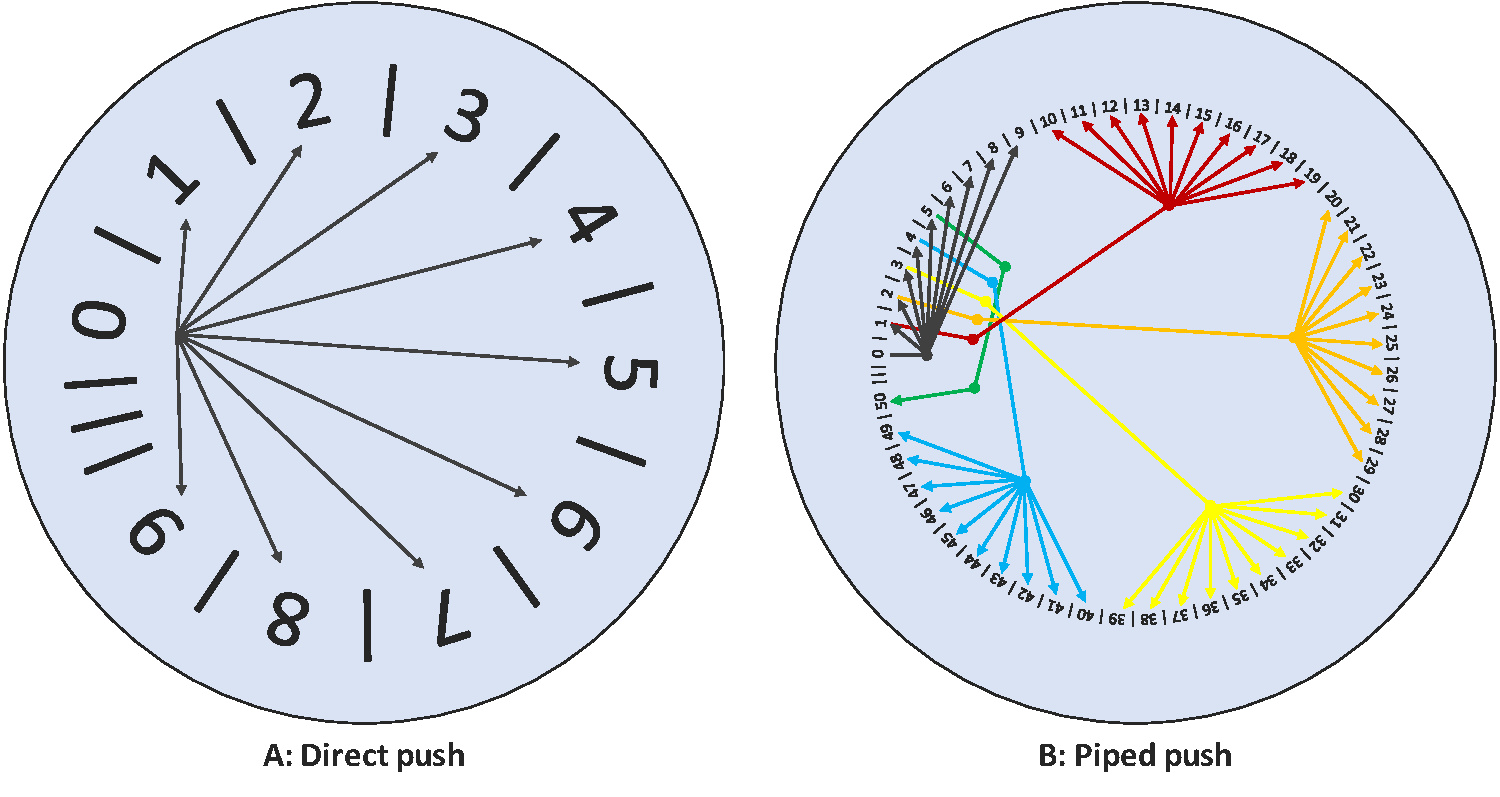
\includegraphics[width=.95\linewidth,keepaspectratio=true]{contents/images/PeeringUpdateMechanism}
		\caption{Update Mechanism}
		\label{fig:PeeringPushMechanism}
	}
\end{figure}
As each node has several \gls{DNs}, $y$ defines the number of \gls{DNs} (here: '$0 \leq y \leq 9$').
Hence, the node on index \textit{two} updates	
\begin{center}
	$d = x*10+y = 20+y => 20 \leq d \leq 29$
\end{center}	
the nodes from $20$ to $29$.
Consequently, the node on index \textit{four} updates the nodes $40$ to $49$ and
the node on index $55$ updates the nodes $550$ to $559$. \\
Even if a node has poor connectivity, this source-drain mechanism reduces the network traffic being the \gls{LN} tremendously from $n$ down to \textit{nine}.
A drawback of this \gls{DNs} variation are offline nodes, which have to serve other \gls{DNs}.
If e.g. node \textit{six} is offline, the nodes to be consulted by \textit{six}, $60$ to $69$, and their \gls{DNs} will miss the latest turn's update.
Nevertheless, the round-robin alternation leads to changing update paths with every turn. \\
During the next alternation, the offline node \textit{six} becomes the index \textit{five} and hence, now fails to update nodes $50$ to $59$, whilst $60$ to $69$ are consulted by the new node, which just moved on index \textit{six}.
Again, this stiff and predefined solution is not possible in traditional \gls{BC} solutions.
Changing peers and undefined source nodes prevent this kind of peering in other \gls{CM}s.\\
The so far explained push mechanism can be called vertical-push, as it establishes pseudo layers (Figure \ref{fig:PeeringPushLayered}).
Here the \gls{LN} represents the (\textit{1st}) source layer (Figure \ref{fig:PeeringPushLayered}: Node 0) and
it's \gls{DNs} are contextualized on the \textit{2nd} layer (Figure \ref{fig:PeeringPushLayered}: Nodes \textit{one} to \textit{nine}).
The push mechanism follows a traditional tree structure (Figure \ref{fig:PeeringPushLayered}: Black arrows) and offers the corresponding '$h = log10(x)$' to calculate the number of hops needed to transport an update from the \gls{LN} to any index $x$.
\begin{figure}
	\centering{
		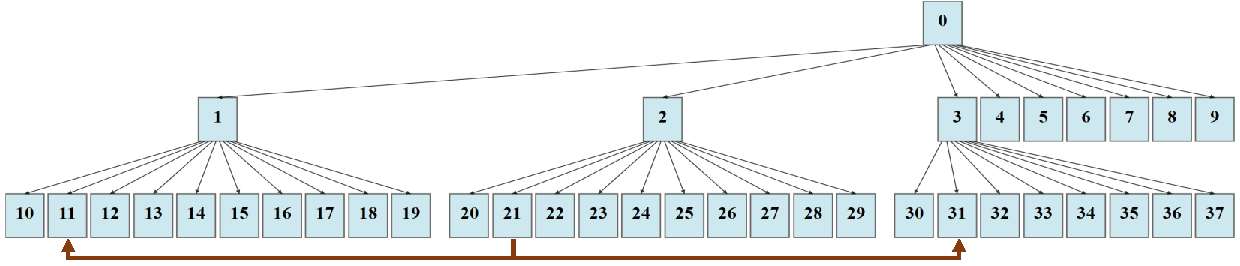
\includegraphics[width=.95\linewidth,keepaspectratio=true]{contents/images/PeeringPushLayered}
		\caption{Pseudo layers of peering by pushing}
		\label{fig:PeeringPushLayered}
	}
\end{figure}
Additionally, further sample enhancements such as \textit{horizontal pipes}, \textit{Jump pipes} and \textit{full-push} are described.
\begin{enumerate}
	\item Horizonal pipes: \\
	A \textit{horizontal pipe} pushes information on the same layer from one node to another, e.g. from node $21$ to the nodes $11$ and $31$ (Figure \ref{fig:PeeringPushLayered}: Brown arrows).
	If the nodes $11$ and $21$ have not already received,
	the designated upper level node(s) may be asked to confirm the horizontal update.
	Alternatively, the neighboring nodes may be asked as well.
	
	\item Jump pipes: \\
	Jump pipes skipping a level may occur, if any source node does not reach a distribution node.
	Then, e.g. node \textit{zero} is not able to reach node \textit{two} and therefore pushes the update directly to the nodes $20$ to $29$.
	
	\item Full push: \\
	As stated before, pushing all updates to the whole network might be expensive for the \gls{LN}, especially in large networks.
	Nevertheless, in contrast to loosely coupled \textit{public permissionless} networks,
	in \gls{PoT} the \gls{LN} is expected to knows all the network's nodes.
	Therefore, some circumstances may benefit a 'full push'-solution (compare \textit{Aura} and \textit{Clique} in \citet{Angelis.2018}), such as transition blocks or any block which demands immediate consultation.
	Especially, the handover-/finalizing block is a crucial block for the \gls{LN}, as it marks the end of all in this turn written data.
	If this block is delivered, it sends all missed data to any receiving node.
	Hence, unattended and dropped behind nodes receive a fresh input.
	Additionally, once the \gls{LN} has finished its turn, it is not occupied anymore.
	Therefore the node is able to distribute the data without performance loss (during its turn) throughout the network.
\end{enumerate}
Further mechanisms to fix \textit{update prevention}, caused by offline nodes, remains implementation dependent.

\bigbreak

\noindent Concluding, the sample \textbf{pull-mechanism} offers to skip updates (e.g. pulling only every second turn) and therefore reduces network traffic throughout.
Obviously, if an increased pulling is not conducted, this comes to the cost of outdated data.
The latter is bad for spontaneous events, such as randomization and trigger events.
The other way around, much consultation in vain is happening as pulls are conducted without receiving new data.
An implementation dependent trade-off has to be found. \\
The key benefit of \textbf{push-mechanisms} is the ability to provide updates fast whilst reducing the traffic for requests.
Especially randomization and trigger events, as far as needed, demand for throughout high availability of every node
and therefore favor push based peering solutions.
Nevertheless, loosing the network is supposed to be one of the major threats for \gls{BCT} systems.
Therefore, pull mechanisms are an essential part of the network, especially if nodes loose connectivity.
Finally, a push-mechanism appears to be superior to a pull-mechanism, nevertheless it was shown
that \gls{PoT} can generally be operated by a pull-mechanism as well. \\
Additionally, the two mechanisms are not mutually exclusive and may be combined as needed.
Thus, a mix of both is generally recommended.
Hence, it is implementation dependent when the network is assumed to be lost e.g. if there was no update from the last three writing nodes.
Here it should be aware that \gls{BCT} solutions assume that nodes have an extrinsic (e.g. \gls{PoW}) or intrinsic (\gls{PoT}) desire to stay online.
Consequently, it is assumed that the peers next to the leading nodes behave in a way offering high availability.
Still, it has to be assumed that mobile clients only offer a reduced bandwidth.
This behavior is unlikely for fat clients, traditionally linked with mining in other \gls{CM}s.
Nevertheless, if nodes are represented by consumer systems, mobile clients are assumed to have an increased online availability
compared to desktop systems, because mobile clients are turned of or cut from the network (flight-mode) only on seldom occasion.
Smartphones, being usually switched on during mobility, strengthens this assumption.
In this regard, if not addressed by lower level peering, mobile clients might change their network address more often.
If this case is applicable, a higher interconnection may be needed.
After all, it is recommended to first design the upper level application to assemble the needed characteristics of \gls{PoT}.
With these characteristics the effective features regarding consultationfull and consultationless interconnection and consequent peering can be decided upon. \\
As the general information flow is supposed to be solved without a superior ledger,
other questions raises regarding \gls{CF}, Byzantine Fault Tolerance and so forth. \\



\FloatBarrier



\section{CAP Theorem measurement}
\label{sec:CAPtheorem}
\begin{figure}[!b]
	\centering{
		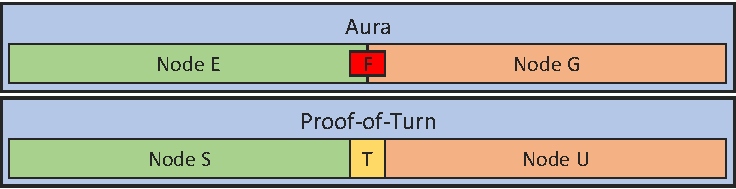
\includegraphics[width=.95\linewidth,keepaspectratio=true]{contents/images/PermissionTransition}
		\caption{Permission Transition}
		\label{fig:PermissionTransition}
	}
\end{figure}
\noindent The CAP theorem (see: \citet{Brewer.2012}) is one of the most important models to describe distributed database systems.
"The CAP theorem asserts that any networked shared-data system can have only two of three desirable properties.
However, by explicitly \textit{handling partitions}, designers can optimize \textit{consistency} and \textit{availability}, thereby achieving some trade-off of all three" \cite[23]{Brewer.2012}.
\citet{Angelis.2018} compare in their paper two \gls{PoA} implementations, \textit{Aura} and \textit{Clique} with \gls{PBFT} regarding the CAP theorem. \\
They claim that \textbf{consistency} is achieved, when forks are avoided \cite[6]{Angelis.2018}.
Consequently, consistency in the context of \gls{BCT} is represented by instant consensus finality \cite[6]{Angelis.2018}.
\textit{Aura} fails in this matter as glitches might occur during the transition from one \gls{LN} to another, resulting in \textit{no consistency} \cite[7]{Angelis.2018}.
In detail, the time frames to write blocks in \textit{Aura} are shown by \textit{node E} and \textit{node G} (Figure \ref{fig:PermissionTransition}: Aura).
\textit{Node G} is the successor of \textit{node E}.
Due to exact timing, \textit{node E} could propose a block within the time slot \textit{F} (Figure \ref{fig:PermissionTransition}: Aura), wherein any node of the network may already assume \textit{node G} to be the \gls{LN}.
The \textit{Aura} client fails and the conflict is not solved.
\textit{Clique} does not meet \textit{consistency} as well, as several nodes are allowed to write simultaneously.
Solving this issue using the Ethereum GHOST protocol leads to \textit{eventual consistency} \cite[8]{Angelis.2018}.
In this regards, \gls{PoT}'s \textit{consistency} can be considered high because of the before mentioned \textit{transition times} (Figure \ref{fig:PermissionTransition}: Proof-of-Turn, T).
\begin{figure}
	\centering{
		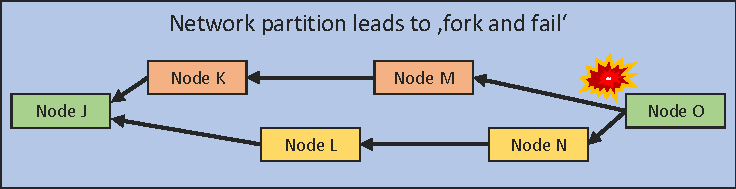
\includegraphics[width=.95\linewidth,keepaspectratio=true]{contents/images/PoT_Fork}
		\caption{Network Partition in PoT}
		\label{fig:PoTfork}
	}
\end{figure}
First, a \textit{transition time} is only needed if \textit{node S} uses the full turn time.
\textit{Node U} has to assume that the writing permission will not be received before 'turn time plus transition time' is over.
Second, \textit{transition time} prevents the network from assuming different leaders due to \textit{time skews}.
Therefore the duration of each \textit{transition time} has to be chosen large enough to compensate inaccuracies of the client's time protocols.
After all, \gls{PoT} does not need as precise timing as \textit{Aura} or \gls{PoET}. \\
Viewing from another angle, a \gls{BC} "[...] is \textbf{available} if transactions submitted by clients are served and eventually committed, i.e. permanently added to the chain" \cite[7]{Angelis.2018}.
Following \citet{Angelis.2018}'s example of the \gls{PBFT} mechanism, \gls{PBFT} stalls sometimes giving up \textbf{availability} to achieve \textit{consistency} \cite[8]{Angelis.2018}.
The stall occurs, when the network can not agree on a \gls{LN} or a transaction proposed by any node is not added to the \gls{BC} for a long time.
Assuming \gls{PoT} as a 'networked shared-data system' it prevents writing by every client simultaneously, sacrificing \textbf{availability}.
If the \gls{LN}, by chance, has no network connection and is therefore not available, \gls{PoT} stalls (temporarily).
Data from the \gls{LN} can not be written to the \gls{BC} by other nodes, as other nodes can not sign the blocks accurately.
Arguing that the other nodes are not willing/allowed to write would break the 'networked shared-data system'-assumption and makes the CAP Theorem classification obsolete.
It would result in a circulating centralized server. \\
Last, when "[...] a \textbf{network partition} occurs, authorities are divided into disjoint groups in such a way that nodes in different groups cannot communicate each other" \cite[7]{Angelis.2018}.
This scenario is shown in figure \ref{fig:PoTfork}, where the network is split into two groups, orange (Node K \& node M) and yellow (Node L \& node N).
The two groups do not see each other and assume that the other side is 'just absent'.
Now, node O two distinct branches of the \gls{BC}.
If these branches represent different game states, they may be mutally exclusive.
As game states depend on each other, e.g. in \hyperref[def:RftS]{RftS}, node M unknowingly sends a fleet from a planet which has been conquered by node L just before.
The resolution of such forks can only be solved within an upper layer and might demand a reset of the \gls{BC} to any previous block/state.
In the worst case an upper level game is broken and has to be stopped.
The resolution of forks by the game layer remains implementation dependent.
Concluding, regarding the CAP Theorem, \gls{PoT} fails partition tolerance. \\
Along these thoughts, \citet[7-8]{Angelis.2018} categorize the \gls{PoA} implementations \textit{Aura} and \textit{Clique} as well as \gls{PBFT} into the CAP triangle.
\begin{figure}
	\centering{
		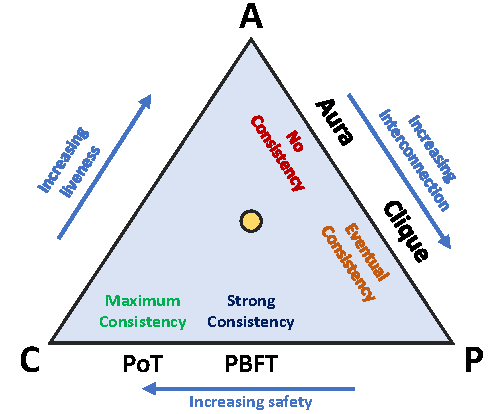
\includegraphics[width=.72\linewidth,keepaspectratio=true]{contents/images/CAPTheorem2}
		\caption{Mechanisms regarding the CAP Theorem (Adapted from \citet{Angelis.2018})}
		\label{fig:CAPTheorem}
	}
\end{figure}
If \gls{PoT} was categorized as a \textit{circulating centralized server}, as all nodes except the \gls{LN} are considered to be silent throughout,
it would be positioned in the middle of the triangle (Figure \ref{fig:CAPTheorem}: Yellow circle).
If \gls{PoT} was categorized with \textit{eventual consistency}, as a pull mechanism does not always provide the newest data,
it would be in the same area as \textit{Clique}.
If \gls{PoT} was categorized as handling \textit{network partition} well, as the upper level use case was only a dumb storage solution without constraints within pushed data,
it would be similar to \gls{PBFT}.
Nevertheless, following the argumentation, \gls{PoT} is added, as shown in figure \ref{fig:CAPTheorem}.



\FloatBarrier

\section{Forks \& transition blocks}
\label{sec:TransitionBlocks}

In any \gls{BCT} certain problems occur, such as forks (\citet[60]{Butijn.2020}; \citet[54]{Dib.2018}).
A fork takes place if there are two mutually exclusive continuations of the approved \gls{BC} \cite[22]{Yuen.2019}.
The network has to decide which trail is going to be followed (\citet{Courtois.2014}; \citet{Ewerhart.2020}) or has to start again from the last legitimate (non exclusive) block \cite[3-4]{FinlowBatesK..2017}.
It has to be mentioned that this section is not about \textit{soft-/hard forks}
on the \gls{BC}'s \gls{CM}'s protocoll \cite[4-5]{FinlowBatesK..2017}. \\
While most Proof-of-Mechanisms solve this issue using the \hyperref[LongestChainRule]{Longest Chain Rule} (\citet{Courtois.2014}; \cite{Nakamoto.2009}),
\gls{PoT} insists on following the rules regarding timing.
The blocks which can only be written by the \gls{LN} have to be pushed within the given time frame of the turn (see figure \ref{fig:PermissionTransition}: PoT).
Hence, the race condition is not dependent on computation power, but on a valid identity regarding time.
Having the turn grants authority to write.
At this point, \gls{PoT} could be classified as a special type of \gls{PoA}.
If a fork is detected, there are basically \textbf{four choices}: \\
\textbf{First}, the branches are soft exclusive, as the upper level software
allows to \textit{merge the branches} without dispute (\citet[7-8]{RanchalPedrosa.2020}; \citet[4-5]{Wang.2018}).
The data from one of the two branches is encapsulated by the recent \gls{LN}, signed and appended on the other branch.
Once merged, data from both branches are \gls{CF} on the main chain and the \gls{LN} continues with its own data.
\textbf{Second}, the branches are \textit{mutually exclusive} .
Nevertheless, encapsulation takes place to regain a consistent main chain.
Next, a dispute has to be raised to decide upon \gls{CF} and invalidation of the questionable parts.
This triggers a network vote on which (on-chain) fork has to be continued.
Herein might be decided on a reset, which resolves in a replay of some turns.
Alternatively, \textbf{third}, a node (or transition block) is \textit{chosen to be continued from},
terminating in a (soft) loss of some turns which will have to be conducted again.
This behavior equals \gls{PoW}'s \textit{Longest Chain Rule} \cite[2]{Ewerhart.2020}
as some transactions/blocks were computed in vain \cite[3-4]{FinlowBatesK..2017}.
\textbf{Fourth}, the worst case for the \gls{LN} originates from a failed vote - now
the \gls{LN} has to \textit{decide on its own} which branch to continue.
The easiest way for the \gls{LN} would be to just choose one branch (randomly, internally).
The drawback is that lacking consultation prevents consent and endangers the \gls{CF} of the \gls{LN}'s data.
Likewise, the decision can be made using a randomization call - which is the most interactive version, raising participation.
The other possibility is to choose the chain which implies the highest loyalty e.g. the most turns.
It is important to mention that the branch offering the most turns is not necessarily the one with the most blocks.
Consequently, the \textit{Longest Chain Rule} is not applicable here.
\begin{figure} [!b]
	\centering{
		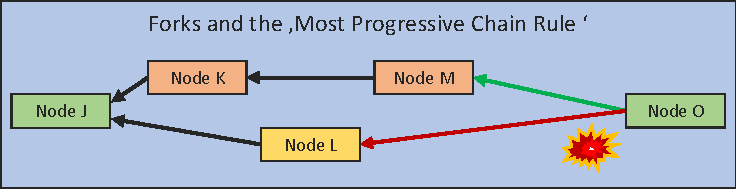
\includegraphics[width=.95\linewidth,keepaspectratio=true]{contents/images/PoT_Fork_Progress}
		\caption{Most Progressive Chain Rule}
		\label{fig:PoTForkProgress}
	}
\end{figure}
Nevertheless, the chain which represents the most turns, is the one which offers the highest resilience against network votes (e.g. regarding invalidation).
The more stakeholders can be assumed for a branch, the higher the possibility for a positive network vote.
Concluding, the chain, continued by the \gls{LN}, is the one representing the most progress regarding turns (Figure \ref{fig:PoTForkProgress}).
After all, to give this scheme a name, \gls{PoT} uses a '\textit{Most Progressive Chain Rule}' instead of the \textit{Longest Chain Rule}. \\
Here, it is likely that a loyalty based approach is superior to a randomization based approach and randomization is only chosen, if the forks offer the same loyalty factor.
The node could also use the values from the failed network vote to influence its decision (slightly). \\
Last, here is a \textbf{fifth} negligible solution:
As creating new blocks in the \gls{PoT} \gls{CM} is cheap, a node could follow several branches.
This solution creates forks even if none has occurred in the first place.
Each node would fork from the last some transition blocks, resulting in turns which have to be calculated several times with changing preconditions.
Therefore the latter option is not considered as an option in the first place.
The effective arrangement is implementation dependent. \\
Of course, the validity of a transaction is checked by every other node.
If a block can neither be checked or rejected, as for \hyperref[HiddenTransactions]{hidden transactions}, it is accepted.
Still it does not change the game state, yet.
If one node does not want to accept an open block, voting determines the validity of the written block - \textit{silence infers consent}.
Nevertheless, the probability of a block to be accepted raises with every silent consent or approved check and is finally accepted if it is approved by a defined threshold of nodes.
Of course, silence could infer refusal as well, but first \gls{PoT} assumes online peers and second, if too many peers were offline, the network would stall constantly.
Hence a \textit{silence infers refusal}-approach is strongly discouraged from.
The threshold, for a vote to pass, can be defined as 'a few nodes' or 'the whole network'.
In table \ref{tbl:SumConsensusMechanisms_3} this was marked as \textit{implementation dependent}. \\
The chosen value affects the \gls{BFT}, the \gls{CF} as well as the smoothness of the \gls{BC} as shown in table \ref{tbl:ConsentSmoothness}.
\begin{table}
	\centering
	\begin{tabularx}{0.71\textwidth}{ c | c | c | c }
		\textbf{Consent} & \textbf{Round Robin} & \textbf{\gls{BFT}} & \textbf{Effective} \\
		\textbf{threshold} & \textbf{smoothness} &  & \textbf{\gls{CF}} \\ \hline
 		Low ($\leq 33.3$ \%) & High & Low & Fast \\ \hline
		Medium ($\sim 50$ \%)  & Medium & Medium & Medium \\ \hline
		High ($\geq 66.6$ \%) & Low & High & Slow \\ \hline
		\hline
	\end{tabularx}
	\caption{Consent smoothness}
	\label{tbl:ConsentSmoothness}
\end{table}
\noindent Luckily a high consent threshold does not lead to a freeze,
such as in \hyperref[def:MultiChain]{MultiChain} \gls{BC}s because of the \textit{silence infers consent}-principle.
Even if there is no interaction, the Round Robin procedure proceeds.
Consequently, latest after one full round a block reaches effective-\gls{CF}.
By then it can not be invalidated anymore.
The \gls{CF} is therefore both faster approached and can be realized with a higher threshold than e.g. \gls{PoW},
as \gls{PoW} suffers from a small residue probability to be forked by any computation superpower \cite[4]{Demi.2021}. \\
Blocks which are not supposed to be in discussion are transition blocks, those blocks which pass the turn from one \gls{LN} to the next.
These transition blocks may enable \textit{adaptive turn time} (See section \hyperref[sec:FurtherCharacteristics]{Further Characteristics}) and ensure consistency (figure \ref{fig:PermissionTransition}: PoT).
Therefore, transition blocks can be used for \textit{fast update verification}.
If a node stays offline for longer, it may ask for an update providing the last known block.
But due to forks or \hyperref[sec:DataAllocationImprovements]{Data allocation improvements} that block is not existing anymore.
Instead the requesting node could provide its last transition blocks, which is not allowed to be deleted.
The last known transition block from the requesting node will then become the start block of the delivered update.



\FloatBarrier

\section{Reveal claims \& trigger events}
\label{sec:ClaimsAndTriggers}

These spontaneous transactions were already mentioned at the end of chapter \hyperref[chap:BlockchainInGames]{Blockchain in Games}.
Although it was stated that general mechanism can be conducted using \gls{BCT}, certain examples were left out.
Therefore, three different approaches are presented hereafter (Figure \ref{fig:TriggerEvents}).
Following it is assumed that the turn is on node \textbf{$\alpha$}. \\
Claims and triggers are active transactions conducted by an intervening node (e.g. \textbf{$\beta$}), breaking the regular writing window, to change the outcome of player \textbf{$\alpha$}'s (sub-)move.
Due to the generally asynchronous nature of \hyperref[def:RftS]{RftS} this is not recommended, but still possible within the \hyperref[def:PoT]{PoT} mechanism.
Possible solutions are given in figure \ref{fig:TriggerEvents} (A-C) and range from 'piping a signed block' (A)
over conducting a 'trigger round' (B), up to 'defined detours' (C).
In \textit{case A} signed blocks are piped via node \textbf{$\alpha$} to the \gls{BC}.
\textit{Case B} describes a fast paced network round wherein only triggers can be pushed legally.
In \textit{case C} the writing permission is only actively given to claiming nodes, who write the triggers themselves before handing the writing permission back to node \textbf{$\alpha$}.
\noindent Whilst reveal claims are straight forward and any answer has to be given by the targeting node,
moves which \textbf{might} trigger, offer certain challenges regarding figure \ref{fig:TriggerEvents}:
\begin{enumerate}
	\item A trigger can only be performed by $\beta, \gamma$ and $\delta$ if both, \textbf{possibility} (any kind of resource) and \textbf{will} (to interfere) are given.
	
	\item In case A (figure \ref{fig:TriggerEvents}) nodes $\beta, \gamma$ and $\delta$ have to believe that node \textbf{$\alpha$} received the piped transaction in time and is not actively ignored.
	The same applies to case C. \\
	As the \gls{LN} is generally allowed to ignore other nodes claims, interoperability may fix this issue (Section: \hyperref[sec:Interoperability]{Interoperability}).
	
	\item Depending on the rules, triggers are not performed in line, players wait for others to execute triggers before they use their own resources.
	Hence, triggers are 'not in line'.
	For case B (figure \ref{fig:TriggerEvents}) this would lead to several rounds of consultation.
	Consequently, if not automatically performed, the manual interaction will slow down the game and/or annoy players due to repeated consultation.
	
	\item Additionally, depending on the numbers of players, case B lacks especially from a long freeze-like waiting time
	until all nodes have performed their answer regarding willingness to fulfill a trigger call.
	However, answering automatically, if the resource to pull a trigger is not available, could unwillingly offer vulnerabilities (e.g.: This node is not able to perform any defensive action).	
\end{enumerate}
Bullet point two could be handled by a child-chain storing raised triggers by $\beta, \gamma$ and $\delta$ including their timestamp.
Due to the random character of calls to pull a trigger, this chain would need to rotate fast with PoT or has to use another type of consensus mechanism, e.g. out of the \hyperref[sec:PbC]{proof based} \gls{CM}s.
\begin{figure}
	\centering{
		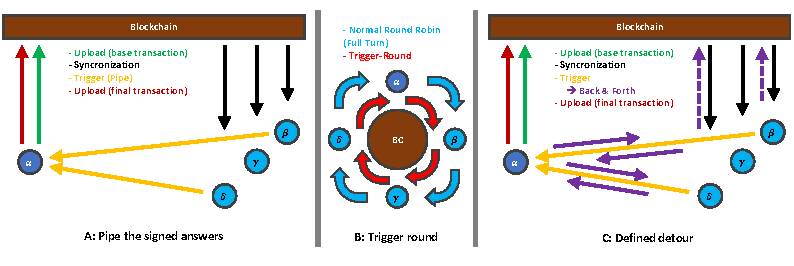
\includegraphics[width=.995\linewidth,keepaspectratio=true]{contents/images/TriggerEvents}
		\caption{PoT: Trigger event mechanisms}
		\label{fig:TriggerEvents}
	}
\end{figure}



\FloatBarrier

\section{Interoperability}
\label{sec:Interoperability}

\begin{figure}
	\centering{
		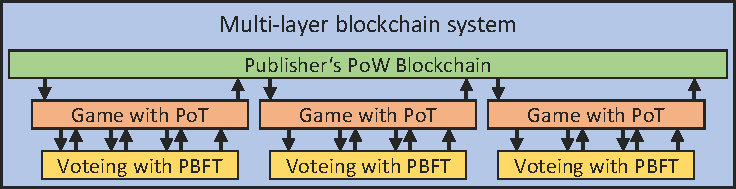
\includegraphics[width=.95\linewidth,keepaspectratio=true]{contents/images/MultiLayerBC}
		\caption{Multi layer BC system}
		\label{fig:MultiLayerBC}
	}
\end{figure}

Except from \citet{Besancon.2019} and \citet{Kraft.2016} there were no papers to be found regarding interoperability of \gls{BCT} for games.
Nevertheless, some implications are given:
Those in the previous chapter mentioned side-chains refer to the before mentioned on-chain, off-chain, child-chain, side-chain and inter-chain methods (\citet{Kim.2018}), see section \hyperref[sec:PerformanceImprovements]{Performance Improvements}.
These methods shall now be inspected for internal and external use regarding interoperability. \\
If not mentioned explicitly, there is no special use case.
Primarily it is focused on multiple layers next to the main-chain. \\
\textbf{First}, internally: If a game wants to augment direct immediate responses in an asynchronous network, preemptive actions have to be taken.
This would include some spare encryption keys or other conducted computation which include network consultation.
It has to be aware that allowing such measures might break the integrity of a game.
For example, computing a randomization in advance lets the player know the chances before actively deciding to take the randomly impacted decision.
Nevertheless, those pre-computed blocks which need consultation, but are not secure to be conducted, shall not be written to the main-chain - just as bloat blocks.
Not conducted turns can be invalidated with a revocation or left open (unrevealed) - just as bloat blocks.
Only those, which are finally used are written to the main chain.
Once all blocks in the side-chain are revoked or written to the main-chain, the side-chain can be deleted.
Moreover, an effective implementation of \gls{PoT} has to decide whether transactions stored in the main-chain only have to be \gls{CF} or at least effectively \gls{CF} (use case dependent).
The latter would call for a child-chain with \gls{CF} blocks/transactions, which is referred to by the main-chain.
The \gls{CF} blocks/transactions in the child-chain are referenced in the main-chain earliest after the defined \gls{BFT} threshold has been passed ($=>$ effective \gls{CF}).
As revoking of \gls{CF} blocks/transactions is supposed to be seldom, the transcription/reference can be done by the emitting node, after the round has passed.
If used, these mechanisms lead to an internal two-layer structure of \gls{PoT}.\\
\textbf{Second}, externally:
This part focuses on \gls{PoT} being an off-chain or side-chain to any other \gls{CM} or \gls{PoT} using any other \gls{CM}s as off-chain or side-chain solutions.
Hence it has to be distinguished between \gls{PoT} being below or above the other \gls{CM}.
For an improved understanding, figure \ref{fig:MultiLayerBC} shows \gls{PoT} in both situations - on
the one hand being a transaction channel child-chain for a \gls{PoW} parent-chain and on
the other hand being a parent-chain for a child chain with \gls{PBFT} functionality (e.g. for voting or trigger events etc.). \\
The below part was already shown by \cite{Kraft.2016}, who uses \gls{PoP} in Huntercoin for game-channels outside a main-chain using another proof-based \gls{CM}.
The other way around would be to fix the  issue of availability shown in by the CAP theorem.
Here, any child-chain offering a simultaneous proposing of blocks would be suitable.
Consequently, dispute resolution by votes and other messages which are of simultaneous nature may be covered with those child-chains, whilst the actual game play is maintained by \gls{PoT}.
A child-chain for votes and disputes could prevent \gls{LN}s from ignoring unwanted messages and enable simple trigger-event resolution
without circumlocutory logic (Section \hyperref[sec:ClaimsAndTriggers]{Reveal claims \& trigger events}).
Last, if needed, a publishers server may be established as a part of any of these chains - the publisher's incentive to do so is consciously left open.



\FloatBarrier

\section{Peer-Fluctuation \& adaptive turn time}
\label{sec:PeerFluctuation}

During the existence of a \gls{BC}, there are multiple reasons for nodes to leave or join the \gls{BC}'s network.
Whilst joining is generally considered an active move, leaving can both be an active operation as well as a passive coincidence. \\
\textbf{Join operations} can be maintained as any node within the network proposes a new node.
Either the network decides whether the proposed node will be added, or a trusted entity (e.g. a publisher's server) may add a node to the network ($n \to n+1$).
The network's (/game's) state predetermines where the node is added regarding the round robin state. 
The new node's index is chosen by the upper level software as it may be inserted at the end of the round or within the next some turns.
In a self organized network using the pull mechanism, without a publisher's server, it may take long to add a new node if no trigger event mechanism is used.
Nevertheless, to prevent two nodes from assuming to be the \gls{LN}, it is discouraged from replacing the recent \gls{LN}  as well as inserting the new node as a successor of the recent \gls{LN}. \\
\textbf{Leave operations} can be conducted by publishing all data the network needs to keep the upper level software running.
This is especially needed in a game's card draw-scenario and likewise situations.
The leaving node is cut out of the round robin and each round progresses faster ($n \to n-1$).
It has to be determined whether a node is allowed to rejoin.
Here, if private keys are shared during the leave operation, a rejoin is only possible using a new identity.
Both, join and leave operations are active operations. \\
Dropping out by (passive) \textbf{coincidence} is possible as well.
For nodes leaving without a trace like software/hardware errors or any longer network connection outage,
the upper level software has to be designed in a resilient way to cover such coincidence (e.g. shared keys for shuffling cards, figure \ref{fig:ShuffleCards}).
If it fails to cover these cases, the \gls{BC} could be hold hostage by any absent node.
As the Round-Robin procedure continues, there have to be mechanisms which lead both, the network and the node to regain the connection.
First, if all nodes are considered fluid parts of a larger network, a static server may help to keep trace as a lost node may ask the static server upon the other nodes of the network.
Alternatively, second, if the lost node is the \gls{LN}, the \gls{BC}'s network could sacrifice the static amount of time of the \gls{LN}'s turn in favor of a likely re-connection.
This action can be seen as the counterpart of 'ending a turn prior to its maturity'.
Both actions are seen as measures of \textbf{adaptive turn time}.\label{sec:AdaptiveTurntime}
The granted amount of time (from minutes to days) as well as punishments after the lost node's re-connection remains implementation dependent.
To find a suitable measure \citet[27]{Laneve.2019}'s claim of \gls{BCT} to be a "risky choice for developers" comes back to mind.
In a gaming context, the other players would have to wait longer during the prolongation.
Still, for in-game experience it is important to reduce waiting times as waiting "[...] is frustrating, demoralizing, agonizing, aggravating, annoying, time consuming and incredibly expensive." \citet{Buffa.1976} as cited in \cite[1]{Maister.1984}.
Consequently chopping down waiting time is considered a key feature.
To solve this deadlock, \gls{BCT} in general seems inappropriate. \\
Nevertheless, following the idea of adaptive turn time, measures such as a \textit{night switch} or a \textit{vacation break} could be implemented as well.
For Pause-by-Consensus votes, some players might not be able to answer manually, as they do not suppose to have their turn.
This is especially true for long termed games with multiple players.
Therefore opt-in, opt-out or predefined answers are recommended.
It has to be aware that a malicious node could pause the game repeatedly if too many nodes give automated positive answers for each prolongation.



\FloatBarrier

\section{Further Characteristics}
\label{sec:FurtherCharacteristics}
This chapter covers further mechanics which can/have to be used to enable certain game characteristics.

\begin{enumerate}
	\item \textbf{Helper Nodes} \label{sec:HelperNodes} \\
	Although most game mechanics can be guaranteed, using \gls{BCT} only, some mechanisms need intervention of external resources/nodes. \\
	In a basic scenario there are no such mechanisms which need strict timing to circumvent race conditions as transition times (figure \ref{fig:PermissionTransition}: Proof-of-Turn) prevent race conditions from delayed network messages.
	However, if transition times are diminished or left out to speed up, additional external resources (figure \ref{fig:MultiLayerBC}: Upper \gls{BC}) may be needed to solve race conditions.
	Still, each additional consultation results in a slower algorithm.
	It is encouraged to just set the transition time appropriately. \\
	Nevertheless, such helping nodes shortcut cumbersome solutions such as randomization and (hidden) card draw.
	A helping node might even be a publishers (central) server.
	Consequently, the publishers server does not host games entirely, but keeps being available for certain services.
	Especially for randomization this may help to meet tight time frames instead of waiting for slow (inactive) peers.
	In this case 'tight' means $\leq5$ seconds to maintain a reasonable user experience. \\	
	Additionally, if no lower level chain (figure \ref{fig:MultiLayerBC}: Lower \gls{BC}) for intervening messages is provided, a central server may be used as a referee in any dispute.
	Any \gls{LN} would therefore not be able to deny transactions/messages with for the \gls{LN} disagreeable content.
	However, this is not seen as a suitable solution, a structure as shown in figure \ref{fig:MultiLayerBC}) should be sufficient for this case and is therefore recommended.
	
	\item \textbf{Shared node resources and cooperative gaming} \\
	The distributed nature of \gls{PoT} enables each player to use several devices to act as one node (\citet{Harkanson.2020}).
	if multiple participants offer the same authorization and authentication parameters, they can be seen as one node (\citet{Karafiloski.2017}).
	Although this feature could be enabled, it has to be considered how the clients are supposed to behave.
	Here, contradicting data has to be avoided as, only one of the devices shall behave as a \gls{LN}.
	If its the player's turn, consequently only the used device shall be consulted to pull from.
	Nevertheless, \gls{BCT} enables cooperative gaming of
	several persons as one player in the game (\citet{Harkanson.2020}).
	The players have to be aware that once granted access rights (private keys) can not be reversed.
	Nevertheless, this feature could enable to play cross platform with many devices (e.g. Computer, Smartphone and Tablet).
	
	\item \textbf{Game session interaction} \label{sec:GameSessionInteraction} \\
	Imagining parallel games of \hyperref[def:RftS]{RftS} with likewise parameters this could allow (given certain parameters) to send a fleet from game A to another game B.
	Here, following figure \ref{fig:MultiLayerBC}, both games might be initiated on the upper level and played on distinct \gls{PoT} \gls{BC}s.
	The sending transaction would include to join the other game's network and become a node in both round robin circles.
	The games do not necessarily need to be in sync and the newly added node (/player) becomes a node following the peer-fluctuation rules of the specific implementation.
	Here, an upper level \gls{BC} as seen in figure \ref{fig:MultiLayerBC} or a helper node for the transition is believed to be necessary.
		
	\item \textbf{Reference Implementation} \label{sec:Reference Implementation} \\
	There are manifold implementation dependent characteristics for a network based on \gls{PoT}.
	\gls{PoT} has to fit the purpose of the business case and has to be set up accordingly.
	The described business case is not part of this document and hence a reference implementation does not fall into place.
	Therefore it is desisted from conducting a reference implementation.
	Nevertheless, table \ref{tbl:PoTparameters} lists parameters to be considered:
	
	\begin{table}[!b]
		\centering
		\begin{tabularx}{0.69\textwidth}{ l | c }
			\textbf{Parameter} & \textbf{Value} \\ \hline
			Nodes & Open ($1$ to $\infty$) \\ \hline
			Turn time & Open ($10$ seconds to several years) \\ \hline
			Maximum block size & $1$ to $\infty$ transactions \\ \hline
			Transition times & 1 to 10 seconds \\ \hline
			Finalizing blocks & Boolean \\ \hline
			Handover blocks & Boolean \\ \hline
			Peering & Push- \textbf{vs.} Pull- \textbf{vs.} Mixed-mechanism \\ \hline
			External resource & None \textbf{vs.} Server \textbf{vs.} Upper level \gls{CM} \\ \hline
			Sub-Chain & Boolean (+ chosen \gls{CM}) \\ \hline
			Votes (/\& Disuptes) & Boolean (+ define rules) \\ \hline
			Randomization & Boolean (+ define rules) \\ \hline
			Adding nodes & External resource \textbf{vs.} Self maintained \\ \hline
			New node's index & Start, Next, End, etc. \\ \hline
			Adaptive turn time & Boolean (+ define rules) \\ \hline
			Multiple devices & Boolean (+ define rules) \\ \hline
			\hline
		\end{tabularx}
		\caption{Parameters of \gls{PoT}}
		\label{tbl:PoTparameters}
	\end{table}
	
	
	
\end{enumerate}



\FloatBarrier

\section{Attack Vectors}
\label{sec:AttackVectors}

Now, some general attacks on \gls{BCT} are described.
Consequently, attacks against popular \gls{CM}s are described and the applicability on \gls{PoT} is given.
Additionally, some attacks special to \gls{PoT} are described as well. \\
An attack shall be considered any hostile behavior which might impact negatively on single nodes or the network itself.
It has to be distinguished between \textit{inside} and \textit{outside} attacks.
Here it is asked whether the saboteur is part of the network or not.
Moreover it has to be distinguished between tricking the upper level software and destroying the \gls{BC}'s network.
\bigbreak
\begin{enumerate}	
	\item \textbf{Byzantine Fault Tolerance} \\
	As this is one of the most discussed topics (\cite{Dib.2018}; \cite{Khan.2020}; \cite{Gramoli.2017})
	on the \gls{PoW} approach, it has to be mentioned here.
	As \gls{PoW} is designed to be used in a public permissionless (Table \ref{tbl:BlockchainNetworkTypes}) environment 
	wherein all nodes are able to enter and leave freely \cite[8]{Nakamoto.2009},
	an attacker with computational superpower (likewise the majority of CPU power)
	could take over the network (\citet[8]{Nakamoto.2009}; \citet[4]{Demi.2021}). \\	
	The nature of \gls{PoT} is completely different here, first \gls{PoT} is supposed to be used in private/public hybrid/permissioned networks.
	Stil,l proposing new nodes is possible.
	Second, instead of CPU power, the number of controlled nodes is the key for fraud in \gls{PoT}.
	The threshold which marks the \gls{BFT} for \gls{PoT} as described in section 'Consensus finality and Byzantine Fault Tolerance' marks the number of nodes needed to become the networks superpower.
	Once archived to control a share of network nodes above the threshold, lets the attacker vote (and kick) in any wished direction.
	The network has to maintain that such majorities are prevented.
	Still, a \gls{BC} network 'dies' when one all nodes have left.
	Any added node is a threat to the voting power of the other nodes.
	Hence, the upper level software has to define rules for joining nodes.
	
	\item \textbf{Benign faults} \\
	Next to the \gls{BFT}, benign faults are a source of inequality and injustice.
	Here "[...] leader misbehaviours can be caused by benign faults (e.g., network asynchrony, software crash) [...]" \cite[4]{Angelis.2018}.
	Although these benign faults are no attack in the traditional sense (\citet{CharronBost.2009}), they endanger the upper level software to stall (\citet[8]{Angelis.2018}; \citet[7]{Greenspan.2015}).
	As benign faults can barely be distinguished from e.g. 'unavailability on purpose', each implementation has to draw a line between the two cases.
	
	\item \textbf{Nothing at stake, long range and transparent forging} \\
	\cite{Lin.2017} describe two flaws of \gls{PoS}, the \textit{Nothing at stake} attack as well as the \textit{long range} attack.
	Both attacks are applied from inside the network.
	The \textit{Nothing at stake} attack is incentivized by cryptocurrency tokens from proposing a block even if there is no data to be written \cite[301-302]{Lin.2017}.
	\gls{PoT} does not suffer from this as block generation does not offer any cryptocurrency token rewards. \\
	The \textit{long range attack} derives from the \textit{Longest Chain Rule} and an attacker
	who once had a high amount of computing power being able to rewrite the chain later on \cite[302-303]{Lin.2017}.
	\gls{PoT} is resilient against this attack as well, as the data written by a node can only reflect the own turn's transactions.
	As long as the integrity of other nodes is not broken (e.g. published private keys), there is no way for an attacker to augment their moves.
	It has to be mentioned that \gls{PoT} does not rely on a \textit{Longest Chain Rule}, but rather on a \textit{Most Progressive Chain Rule}, which is an adaption of the \textit{Longest Chain Rule}. \\
	Last, some \gls{CM}s such as \gls{PoS} allow to propose the next \gls{LN}.
	If this is possible, a subgroup of nodes is able to pass the \gls{LN} within their peers, which is called \textit{transparent forging} \cite[302]{Lin.2017}.
	Due to the Round Robin procedure of \gls{PoT}, \textit{transparent forging} is not applicable.
	
	\item \textbf{Integrity of nodes} \\
	As details of encryption are seen out of scope, security of symmetric and asymmetric encryption are supposed.
	Still, the loss of the private encryption key(s) is critical to the integrity of any node.
	Once an attacker obtains access to the private key, the nodes identity can be augmented and used in hostile manner.
	Except the loss of the private encryption key(s), \gls{PoT} seems secure on outside attacks regarding integrity.
	Likewise, \citet[251]{Douceur.2002} describes the 'Sybil Attack' wherein large-scale "[...] peer-to-peer systems face security threats from faulty or hostile remote computing elements".
	Here, if "[...] a single faulty entity can present multiple identities, it undermining this can control a substantial fraction of the redundancy." \cite[251]{Douceur.2002}
	Hence, the integrity has to be kept throughout.
	Additionally, \citet{Douceur.2002}'s claim reflects the risk of \gls{BFT} being captured by an entity,
	which represents the majority in a vote through multiple controlled network nodes.
	
	\item \textbf{Timing} \\
	Revisiting the \gls{PoA} client \textit{Aura} from section \hyperref[sec:CFandBFT]{Consensus finality and Byzantine Fault Tolerance},
	malicious \gls{LN}s could try to post their blocks as near to the end of their writing permission as possible to break the algorithm.
	Of course this is considered an inside attack with the implication to break the network.
	This flaw is prevented in \gls{PoT} if \textit{transition times} are enabled.
	
	\item \textbf{Silencing nodes} \\
	The prevention of service of any node of the network can be accomplish by any (larger) entity.
	The idea can be abstracted from a single attacking device accomplishing \textit{Denial of Service}, therefore the term \gls{DDoS} is used.
	\gls{DDoS} can be both of internal and external nature (see \citet{Wu.2010}). \\
	\citet[72]{Johnson.2014} take a look at Bitcoin (\gls{PoW}) mining pools and see both potential and incentive to use \gls{DDoS} to gain competitive advantage over other mining pools.
	\gls{PoW} does not assume any node to provide a block, hence  the attack only harms the single node without hurting the remaining network.
	In \gls{PoT} the targeted node has to be distinguished between the \gls{LN} and any other node. \\
	Assuming that there is no data the network needs from the targeted node to continue, the \gls{DDoS} attack is only harms the state of the single node (update prevention).
	This is applicable if the targeted is not the \gls{LN} and does not have to deliver data (e.g. trigger/card draw/randomization). \\
	The other way around, if the targeted node is the \gls{LN}, the network is targeted entirely, as the progression stalls until the \gls{LN}'s turn is over.
	Still, information which has to be provided to the network by the \gls{LN}, can not be served. \\
	It can not be avoided, that the distributed and interconnected structure of \gls{BCT} has to expose the needed network address information, which is needed to conduct the attack.
	The general solution would be to guarded nodes from each other by a central server, abstracting the network addresses, but this breaks the \gls{BCT}'s paradigm.
	Moreover, the \gls{DDoS} could follow the round robin sequence and target one node after another, silencing the (whole) network.
	Nevertheless, if detected and once the attack is over, the round robin could be reset and continued from the last agreed state.
	
	\item \textbf{Double spending problem} \\
	One of the key problems \gls{PoW} solved is the ability to spend assets/tokens in distributed systems twice \cite[1]{Nakamoto.2009}.
	\gls{PoT} is able to guarantee this as well.
	If a node does not comly given \gls{SC}s, the block/transaction is invalidated by vote and does not reach \textit{effective} \gls{CF}.
	Consequently, the published information which uses \gls{PoT} has to deliver transparent data with every transaction.
	The double spending problem arises when hidden transactions become part of the upper level software.
	In this concern, \citet[56]{Dib.2018} state that "[...] it is always possible to add encrypted data using the recipients public key,
	but then the validators cannot verify the semantics of the transaction (e.g., double spending) [...]".
	Therefore, specific (upper level) implementation has to solve related issues.
	
	\item \textbf{Effective network split} \\
	This refers to a node, sending different data to different parts of the network, resulting in a forced fork.
	This could either happen, \textbf{first}, due to lost identity or team gaming with consequent simultaneous gaming or \textbf{second} hostile emitted blocks by a single node.
	Now "[...] some of the nodes of the blockchain recognize a node as the next block writer,
	while other nodes recognize another node as	the next block writer" \cite[22-23]{Yuen.2019}.
	All three scenarios can be detected by the network as long as the network rechecks the last (transition) block of each \gls{LN} to deliver equal fingerprints (Hashes) on each receiving node.
	Possible resolutions are described in section \hyperref[sec:TransitionBlocks]{Forks \& transition blocks}.
	Hence, consistency can be maintained by preventing network partition.
	
	\item \textbf{Data flooding} \\
	Assuming \gls{PoT} to be a lightweight algorithm for mobile games (e.g. on smartphones) and offering the possibility to write bloat blocks,
	enables to flood the network until some nodes have to drop out of the game due to allocated storage constraints.
	The mechanisms like pruning bloat blocks or meta-state blocks, wiping the history, are countermeasures but can not be seen as all-embracing solution.
	Depending on the final use case, a maximum write permission may be needed as well.
	It has to be mentioned that a limit (rule) may be broken if the network decides it in a vote (changes the rule).
	Nevertheless, single nodes may clean for themselves to keep the 'important' parts of the \gls{BC}.
	Thresholds for both the limit and the vote remain implementation dependent.
			
\end{enumerate}

\noindent Further, more technical, attacks on \gls{BCT} can be found in \cite{Min.2019b}.
As \citet{Min.2019b}'s attacks can not focus on \gls{PoT} yet, they are out of scope.



\section{Limitations}
\label{sec:Limitations}

First it has to be mentioned that this document is (only) based on theoretical background.
Many assumptions had to be made, as seen in table \ref{tbl:PoTparameters}.
Some of the assumptions, as a reminder, are given in the following:
\begin{enumerate}
	\item Many \gls{BCT} \gls{CM}s, due to their extrinsic incentives of cryptocurrency tokens, prevent offline peers.
	A software publisher has to decide whether intrinsic incentives are satisfactory to provide a network with \gls{PoT}.
	Taking the targeted platform with their consumers into consideration may lead to a decision. \\
	Here, strong tiers alike a company's servers, personal computers and gaming consoles tend to be switched off after a gaming session and might not stay online over a longer period of time.
	Consequently extrinsic incentives are needed. \\
	On the contrary mobile phones, likewise to WhatsApp usage, can be supposed stay online most of the time.
	Hence they do not need to be switched on on purpose.
	Nevertheless, offline nodes, stemming from flight mode during night times might stay a problem for \gls{PoT}.
	
	\item Especially if choosing mobile clients, disk size limit has to be evaluated critically.
	Although new devices may offer excessive resources,
	if the targeted consumers are throughout the whole range of devices, average free resources may drop dramatically.
	
	\item Although \gls{PoT} is considered a lightweight solution among other \gls{CM}s, it is still no solution for 'fast paced' upper level software.
	Transition times, needed to provide throughout consistency may be too long for immediate response.	
	This is especially true for large groups of nodes aiming for simultaneous interaction.
	\gls{PoT} is primarily designed for (long term) asynchronous data transfer.
	
	\item \gls{PoT} is not supposed and not able to reduce publishers fear of cloned replicas from open code due to \gls{SC}s or unencrypted shared data for re-engineering.
	The incentive to save maintenance costs on servers have to suffice to cover re-engineering risks.
	Additionally, not updated clients, assuming different parameters, may lead to incompatibilities.
	Changing rules (\gls{SC}s or parameters) after a \gls{PoT} \gls{BC} has been initialized is not recommended.
	Concluding: Once a software using \gls{PoT} is released, the advantage from \gls{PoT} are only the reduced network/server costs.
	
	\item Less about \gls{PoT} and more about games on \gls{BCT}, distributed systems without fallback option are critical for long term usage.
	This can be obtained both from precise timestamps without helper nodes and shared decks of card.
	For the latter, private draws without helping nodes are already cumbersome.
	Hidden draws are not even possible without external help.
	
\end{enumerate}

\section{Interim Summary - Proof-of-Turn}
\label{sec:InterimSummary-PoT}
The implications of \gls{PoT} are promising.
Chosen the right application's use case, \gls{PoT} offers an intelligible framework for fast lightweight and fair distributed gaming experience.
It outperforms \gls{PoW} in terms of speed, whilst still managing to grant equal rights among the peers in comparison to \gls{PoS} and \gls{PoA}.
There is no need for special Hardware as required for \gls{PoET} and no semi-fair additional measure for 'effort' has to be determined as in \gls{PoP}.
Compared to the approaches \textit{Multichain} and \textit{Aura}, freeze-states can be prevented due to granted time frames for turns and the transition time slot between two turns. \\
Still, \gls{PoT} meets a high \gls{BFT}, adjustable to each use case needs,
whilst offering fast \gls{CF} reducing forks and computation in vain.
Last, \gls{PoT} can be seen as open for interoperability as it can be used as a sub-chain as well as it can use other chains below itself, likewise to \citet{Kraft.2016}'s \textit{Game channels}.
Summing up, \gls{PoT} delivers many desirable features for its intended niche. \\
Therefore, after researching and evaluating different \gls{CM}s, the second leading question ..
\begin{center}
	\textit{"What is the best fitting \gls{BCT} \gls{CM} to cover an asynchronous game play scenario?"}
\end{center}
\noindent .. may be answered with "\gls{PoT}" - depending on the application's use case.
Additionally, by shifting the computation requirement from the publisher's central server
to the peers nodes, the research hypothesis .. 
\begin{center}
	\textit{"The \gls{PoT} \gls{CM} leads to a reduction of server running costs for game publishers."}
\end{center}
\noindent .. appears to be admissible. \\

\noindent \textbf{Finally}, after \textbf{first} analyzing recent \gls{BCT} \gls{CM}s,
\textbf{second} researching games, which use \gls{BC}s in their ecosystem
and \textbf{third} presenting a novel \gls{CM}, \gls{PoT},
to complement the existing solutions, a conclusion and outlook is given.

